\chapter{\norm{-e} und \norm{-iu} im Paradigma der starken Adjektivflexion}
\label{ch:adjflex}

In diesem Kapitel wird aufgrund einer Stichprobe aus dem Quellenmaterial das
Paradigma der starken Adjektivflexion mit Fokus auf den Nom./Akk.\ Pl.\ für die
untersuchten Texte rekonstruiert, um sicherzustellen, dass die gesammelten
Belege aus Urkunden des \CAO{} und \KC{}-Handschriften auch
bezüglich ihrer dialektgeografischen Dimension korrekt interpretiert werden.
Indem vorab sondiert wird, ob an bestimmten wichtigen oberdeutschen
Ausstellungs\-orten beziehungsweise in den jeweiligen Handschriften aufgrund
schreibsprachlicher Gegebenheiten überhaupt eine Opposition zwischen \norm{e}-
und \norm{iu}-Formen vorliegt \autocite[vgl.][182]{ksw2}, können Handschriften
sowie Urkundenbelege aus Regionen, in denen dies nicht der Fall ist, im
Vorhinein ausgeschlossen oder mit entsprechender Vorsicht behandelt werden. Das
Paradigma der starken Adjektivflexion, wie es allgemein für das Oberdeutsche zu
mittelhochdeutscher Zeit angesetzt wird, wird in \cref{fig:adjparadgmstr} mit
seinen Synkretismen aufgeführt.

\begin{figure}
\centering
\renewcommand{\arraystretch}{1.5}
\subfloat[pronominale Flexion]{
	\begin{tabular}{| l c c c c c c}
	\hline

	\mr{2}{*}{Kasus}
		& \mc{3}{|c}{Singular}
		%
		& \mc{3}{|c|}{Plural}
		\\

	\cline{2-7}

	%
		& \mc{1}{|>{\centering}m{1.25cm}}{N.}
		& \mc{1}{|>{\centering}m{1.25cm}}{M.}
		& \mc{1}{|>{\centering}m{1.25cm}}{F.}
		%
		& \mc{1}{|>{\centering}m{1.25cm}}{N.}
		& \mc{1}{|>{\centering}m{1.25cm}}{M.}
		& \mc{1}{|>{\centering}m{1.25cm}|}{F.}
		\\

	\hline

	Nom.
		& \mc{1}{|c}{\mr{2}{*}{-eȥ}}
		& \mc{1}{|c}{-er}
		& \mc{2}{|c}{-iu}
		%
		& \mc{2}{|c|}{\mr{2}{*}{-e}}
		\\

	\cline{1-1}
	\cline{3-4}

	Akk.
		& \mc{1}{|c}{}
		& \mc{1}{|c}{-en}
		& \mc{1}{|c}{-e}
		%
		& \mc{1}{|c}{}
		& \mc{2}{|c|}{}
		\\

	\hline

	Dat.
		& \mc{2}{|c}{-em(e)}
		& \mc{1}{|c}{}
		%
		& \mc{3}{|c|}{-en}
		\\

	\cline{1-3}
	\cline{5-7}

	Gen.
		& \mc{2}{|c}{-es}
		& \mc{4}{|c|}{-er(e)}
		\\

	\hline
	\end{tabular}
}

\subfloat[nominale Flexion]{
	\begin{tabular}{| l c c c}
	\hline

	\mr{2}{*}{Kasus}
		& \mc{3}{|c|}{Singular}
		\\

	\cline{2-4}

	%
		& \mc{1}{|>{\centering}m{1.25cm}}{N.}
		& \mc{1}{|>{\centering}m{1.25cm}}{M.}
		& \mc{1}{|>{\centering}m{1.25cm}|}{F.}
		\\

	\hline

	Nom.
		& \mc{3}{|c|}{-Ø}
		\\

	\cline{1-1}
	\cline{3-4}

	Akk.
		& \mc{1}{|c|}{}
		& \mc{2}{|c}{}
		\\

	\cline{1-2}

	\end{tabular}
}
\caption[Starke Adjektivflexion in obd. Schreibdialekten des Mhd.]
	{Starke Adjektivflexion in oberdeutschen Schreibdialekten des
	Mittelhochdeutschen nach \citet[182, Abb. A~3]{ksw2}}
\label{fig:adjparadgmstr}
\end{figure}

\section[Adjektivdeklination im \tit{Corpus der altdeutschen Originalurkunden}]{Adjektivdeklination im \CAO{}}
\label{sec:adjdeclcao}

\phantomsection
\label{phsec:formelhaftigkeit}
Eine automatische Lemmatisierung und Formenbestimmung für alle Token des
\CAO{} auf Basis des \REM{} unter Verwendung des Taggers von
\citet{schmid2019} ist verfügbar
\autocites[vgl.][207]{beckerschallert2021}[155--158]{beckerschallert2022b}. Bei
der Erstellung der Stichprobe für die Rekonstruktion der starken
Adjektivflexion hat sich allerdings gezeigt, dass der Tagger Schwierigkeiten
hatte, die Flexionsendungen korrekt zuzuordnen, insbesondere bei der schwachen
Deklination mit ihren einzigen Flexiven \norm{-e} und \norm{-en}.

\posscite{schmid2019} Tagger hat insgesamt 60.022 Wortformen im \CAO{}
als attributive Adjektiv kategorisiert, darunter auch adjektivisch verwendete
Partizipien. Bei der automatischen Annotation wurde die editorische Abkürzung
\fw{S.} für \wdef{Siegel} 3.321-mal fälschlich als Adjektivform gekennzeichnet.
Von den verbleibenden 56.701 Wortformen wurden 31.805 mit 95-prozentiger
Sicherheit als Adjektiv gewertet. Der Anteil an attributiven Adjektiven und
Partizipien im ganzen Korpus beträgt damit ungefähr zwischen 1,5 und 3\pct{};
sie finden in den Urkunden also eher selten Verwendung. Auffällig häufig kommen
diese Wortformen als Attribute von Präpositionalobjekten in Rechtsformeln vor
\autocites[vgl.][30]{becker2016}:%

\needspace{3\baselineskip}
\begin{itemize}
	\item % \norm{mit \emph{gemeinem} râte}
		\norm{mit \emph{gemėinem} rāte}
		\wdef{mit einvernehmlichem Rat}
	\item \norm{mit \emph{gesamenter} hant}
		\wdef{mit vereinter Hand}
	\item % \norm{mit \emph{verdâhtem} muote}
		\norm{mit \emph{verdāhtem} muete}
		\wdef{mit besonnener Absicht}
	\item % \norm{von \emph{êhafter} nôt}
		\norm{von \emph{ēhafter} nōt}
		\wdef{durch einen rechtsgültigen Hinderungsgrund}
	\item % \norm{ze einem \emph{offenen} urkunde}
		\norm{ƶe ėinem \emph{offenen} urkunde}
		\wdef{zum öffentlichen Zeugnis}
	\item % \norm{ze \emph{rehtem} schirme}
		\norm{ƶe \emph{ręhtem} schirme}
		\wdef{zum rechtmäßigen Beistand}
\end{itemize}

Eine zusätzliche Herausforderung besteht darin, dass die Urkunden für sich
genommen in der Regel zu kurz sind, um alle Formen des Paradigmas zu enthalten.
Für die Hälfte (50,4\pct) der identifizierbaren Ausstellungs\-orte liegt nur
eine einzige Urkunde vor, die laut Ortsverzeichnis dem jeweiligen
Ausstellungs\-ort als einzigem zugeordnet ist. Selbst wenn sämtliche Urkunden
ausgewertet würden, wäre es nicht möglich, für sämtliche Ausstellungs\-orte das
vollständige Deklinationsparadigma zu rekonstruieren. In
\cref{subsec:cao_adjflex_disc} werden daher auch nur einzelne illustrative
Beispiele diskutiert und keine kompletten Paradigmen wie in
\cref{fig:adjparadgmstr} angegeben.

\subsection{Anlage der Stichprobe}
\label{subsec:cao_sample}

Um eine Stichprobe zu erstellen, die den geschilderten Einschränkungen
weitestmöglich entgegenkommt, wurden zunächst diejenigen Ausstellungs\-orte
ermittelt, die eine möglichst große Menge an einzig ihnen zugewiesenen Urkunden
aufweisen und dabei die verschiedenen oberdeutschen Dialekt\-räume abdecken,
auch in Hinsicht auf die auszuwertenden \KC{}-Handschriften (vgl.
\cref{fig:adjstpr_orte}).

\begin{table}
\centering
\caption{Ausstellungs\-orte der Stichprobe}
\begin{tabular}{r l r}
\toprule
Rang
	& Ausstellungs\-ort
	& Urkunden
	\\

\midrule

 1 & Straßburg  & 219 \\
 2 & Zürich     & 143 \\
 4 & Basel      & 117 \\
 5 & Augsburg   &  95 \\
 6 & Salzburg   &  75 \\
 7 & Regensburg &  53 \\
 9 & Wien       &  48 \\
10 & Konstanz	&  46 \\

\midrule

13 & Nürnberg   &  26 \\
15 & München    &  22 \\
22 & Ulm        &  16 \\

\bottomrule
\end{tabular}
\label{tab:adjstpr_orte}
\end{table}

\begin{figure}
\centering
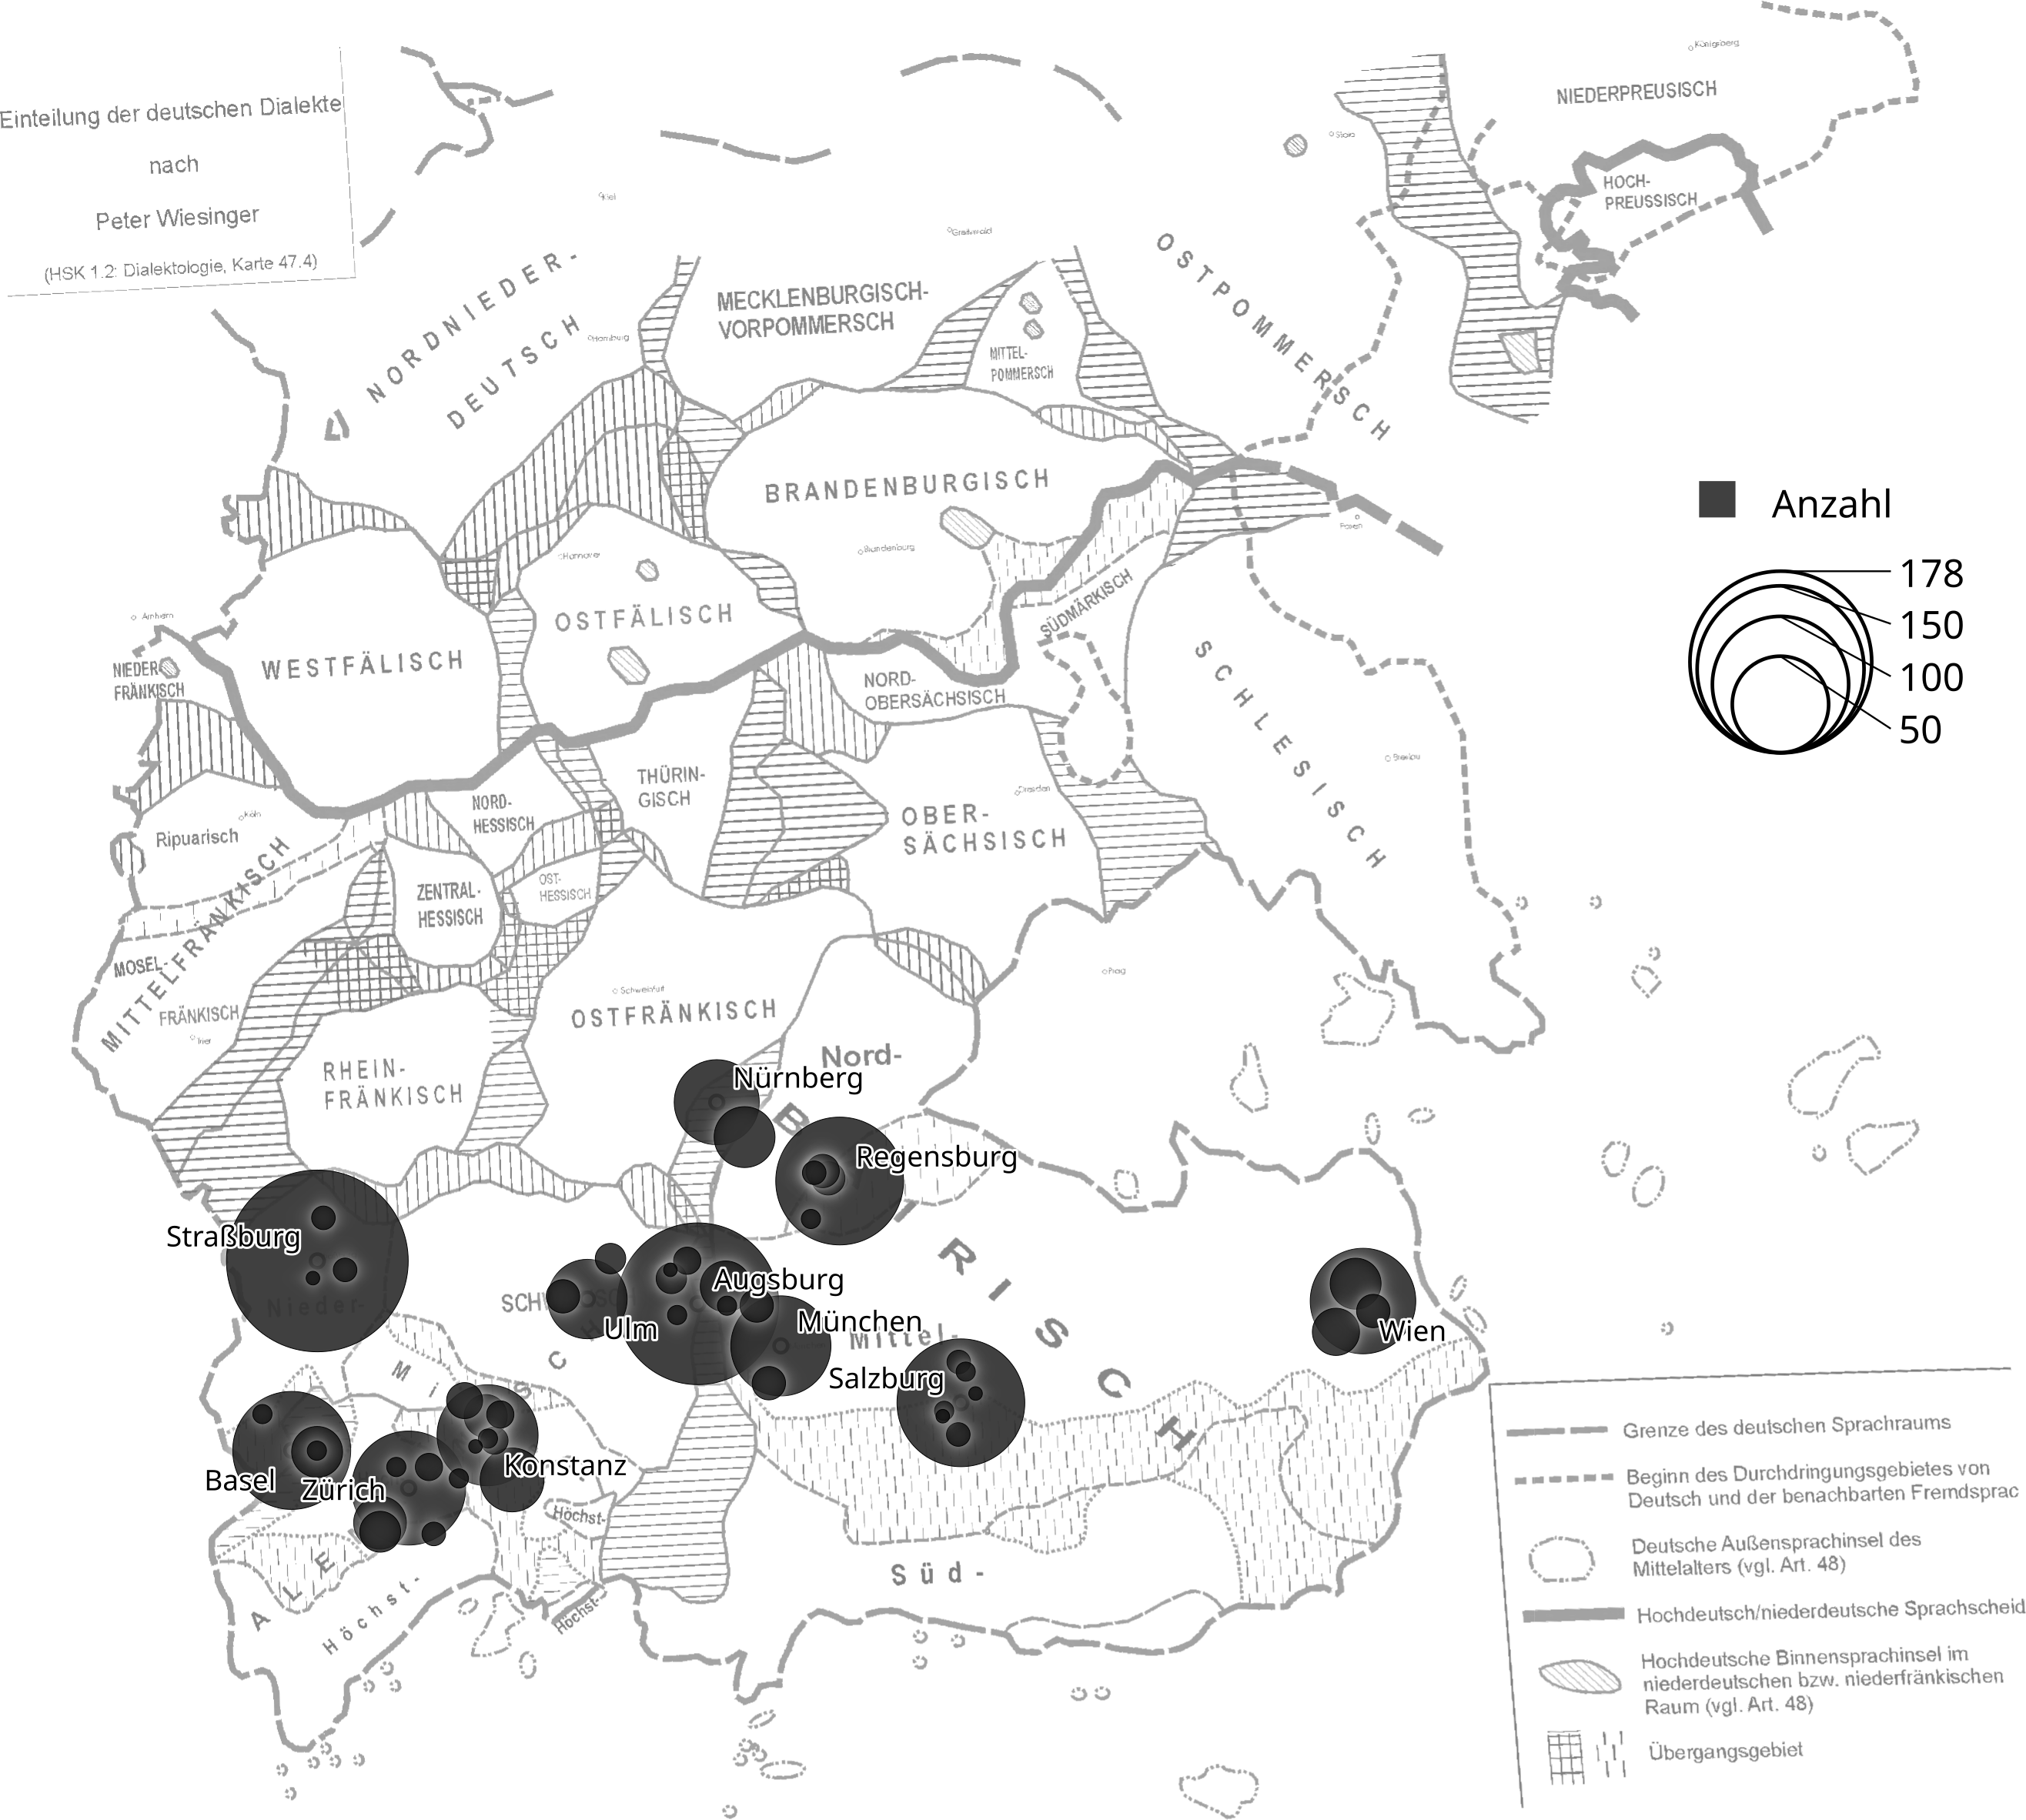
\includegraphics[
	width=\linewidth,
	height=.75\textheight,
	keepaspectratio
]{./assets/grafiken/2021-05-10_adjektivstichprobe_cao.png}
\caption%
	[Menge der Belege pro Ausstellungs\-ort in der Stichprobe zur
		Adjektivdeklination]%
	{Menge der Belege pro Ausstellungs\-ort in der Stichprobe zur
		Adjektivdeklination\nocite{wiesinger1983:rede}}
\label{fig:adjstpr_orte}
\end{figure}

Zusätzlich wurden für alle in \cref{tab:adjstpr_orte} aufgelisteten
Ausstellungs\-orte noch alle weiteren Orte im Umkreis von etwa vierzig
Kilometern (0,25°) hinzugenommen, gerade auch, was Nürnberg, München und Ulm
betrifft, für die jeweils nur wenige Urkunden zur Verfügung stehen. Mögliche
schreibsprachliche Unterschiede zwischen Stadt und Umland sowie die Lage
Augsburgs im Übergangsgebiet vom Schwäbischen zum Bairischen wurden dabei außer
Acht gelassen, zumal hier nicht phonologische, sondern morphosyntaktische
Variation angesprochen wird. Bei der Durchsicht und Klassifizierung der Belege
erwies sich dieser Vorbehalt als unproblematisch.

Für die Anfertigung der Stichprobe ist es nur bedingt nützlich, automatisiert
alle jeweiligen Formen für einen bestimmten Ort ausgeben zu lassen, da die
automatische Wortartzuordnung des Taggers bei Adjektiven nicht zuverlässig
funktioniert und die Wortformenbestimmung teils Lücken aufweist oder ebenso
ungenau ist. Daher wurde zur Auswahl häufiger Lemmata eine Liste aller im
\WMU{} verzeichneten Lemmata mit der dort angegebenen Häufigkeit zurate
gezogen.%
%
	\footnote{Die Liste (mit Stand 2009) wurde der AG~Sprachgeschichte der
	Philipps-Universität Marburg 2013 im Rahmen erster Studien zum
	\CAO{} von Ursula Schulze (†) zur Verfügung gestellt.}
	%
	% U.S. an Jürg Fleischer am 13.02.2013 15:11 Uhr
	% J.F. an Oliver Schallert am 14.02.2013 08:54 Uhr
	% O.S. an mich (Beckerc2@students) am 16.02.13 18:59 Uhr
%
Die Auswahl fiel dabei auf die in \cref{tab:adjsmpwords} aufgelisteten Lemmata.
Um Irrläufer zu vermeiden, wurden nur diejenigen Belege für die einzelnen
Lemmata aus der Datenbank extrahiert, die der Tagger von \citet{schmid2019} mit
mindestens 95-prozentiger Sicherheit dem jeweiligen Lemma zuordnen konnte.

\begin{table}[h]
\centering
\caption{Lemmata der Stichprobe}
\begin{tabular}{l l r l @{\citereset}}
\toprule

Lemma
	& Übersetzung
	& Häufigkeit
	& Quelle
	\\

\midrule

% \norm{êhaft}
\norm{ēhaft}
	& \wdef{rechtsgültig}
	& 105
	& \cite[419--420]{wmu1}
	\\

% \norm{êlich}
\norm{ēlich}
	& \wdef{rechtmäßig}
	& 350
	& \cite[448--449]{wmu1}
	\\

% \norm{ganz}
\norm{ganƶ}
	& \wdef{ganz}
	& 631
	& \cite[549--550]{wmu1}
	\\

% \norm{grôz}
\norm{grōȥ}
	& \wdef{groß}
	& 270
	& \cite[761--762]{wmu1}
	\\

% \norm{guot}
\norm{guet}
	& \wdef{gut}
	& 1.643
	& \cite[770--772]{wmu1}
	\\

% \norm{kleine}
\norm{klėine}
	& \wdef{klein}
	& 116
	& \cite[1011--1012]{wmu2}
	\\

\norm{niuwe}
	& \wdef{neu}
	& 355
	& \cite[1322--1324]{wmu2}
	\\

% % \norm{reht}
% \norm{ręht}
% 	& \wdef{recht, rechtsgemäß}
% 	& 3.330
% 	& \citet[?--?]{wmu2}
% 	\\

\bottomrule

\end{tabular}
\label{tab:adjsmpwords}
\end{table}

Die häufigsten Adjektive, die oft in festen Fügungen wie den eingangs zitierten
auftreten, wurden bei der Auswahl der Lemmata vermieden. Possessivpronomen --
hauptsächlich \norm{mīn} \wdef{mein} (11.250 Belege; \cite[1231--1232]{wmu2})
-- wurden aufgrund ihrer Häufigkeit verwendet, um Lücken aufzufüllen, abgesehen
vom Nom.\ Sg. aller Genera sowie dem Akk.\ Sg.\ N., wo häufig auch eine Form
ohne Flexion steht \autocites[216]{paul2007}[507, 510--511]{ksw2}.
Allerdings ist anzumerken, dass \norm{mīn} \wdef{mein} bisweilen auch im
Nom./Akk.\ Pl.\ M./F. unflektiert auftritt. \citeauthor{ksw2} fassen dies
\blockcquote[510]{ksw2}{im Wesentlichen \textins{als} Resultat der vom Oobd.
ausgehenden Schwa-Apokope} auf. Sie weisen aber auch darauf hin, dass
daneben flektiertes \norm{alle} (mit Schwa) vor unflektiertem
\norm{mīn/dīn/sīn} \wdef{mein/dein/sein} keine Seltenheit in ihrem
Korpusmaterial darstellt. Entsprechende Belege wurden deshalb hier
ausgeklammert.

Für das Alemannische weisen \citet[271, Abb.\ A~47]{ksw2} für
die zweite Hälfte des 13.~Jahrhunderts 10\pct\ flexionslose Formen bei
vorangestellten Adjektiven in Positionen mit regulärem \norm{e}-Flexiv aus,
34\pct\ für die erste Hälfte des 14.~Jahrhunderts; Schwäbisch wird nicht
gesondert verzeichnet. Auffällig bei den Plural-Belegen in der hier
vorgenommenen Stichprobe aus Urkunden des \CAO{} ist, dass
unflektiertes
% \norm{mîn} 
\norm{mīn} \wdef{mein} in allen Fällen vor
% \norm{erben}
\norm{ėrben} \wdef{Erben} steht, wobei das Fehlen der Flexion hier auch auf
Hiatusvermeidung zurückgeführt werden kann.

Noch bestehende Lücken wurden durch manuelle Durchsicht der Urkundentexte zum
jeweiligen Ort gefüllt, wobei darauf geachtet wurde, nach Möglichkeit
wenigstens zwei Belegstellen zu finden und dabei Variation zu berücksichtigen.
Die Annotation der Belege geschah in jedem Fall manuell. Belege, bei denen das
Lemma bei der automatischen Annotation falsch zugeordnet wurde, wurden
übergangen. Die Tabelle im \cref{sec:caoadjquanttab} listet die ausgewerteten
Belegmengen pro Bezugsort mit den hinzugezogenen Ausstellungs\-orten in dessen
Umkreis auf. Im Folgenden sollen kurz die Belege zum Nom./Akk.\ Sg.\ F.\ und
Pl.\ pro untersuchtem Ort charakterisiert werden.

\subsection{Diskussion}
\label{subsec:cao_adjflex_disc}

\paragraph{Straßburg}
\label{par:adjstrassburg}
In Straßburger Urkunden wird regelmäßig kein Unterschied zwischen \norm{e}- und
\norm{iu}-Formen gemacht \cref{ex:adjstrbgregel}. In der Stichprobe sind
außerdem zwei Belege zu
% \norm{êrbære}
\norm{ērbǟre} \wdef{ehrenhaft, edel} mit \lit{-i} für den Nom.\ Sg.\ F.\
enthalten \cref{ex:adjstrbgi_1}. Auch für den Nom./Akk.\ Pl.\ N.\ ist einmal
\lit{-i} in der Stichprobe enthalten \cref{ex:adjstrbgi_3}, sowie viermal
\lit{-u/-û} neben regelmäßigem \lit{-e} \cref{ex:adjstrbgu}, davon ein
Doppelbeleg für \norm{kristenlich} \wdef{christlich} mit \lit{-u} und
\lit{-e} \cref{ex:adjstrbgu_1}. Die betreffenden Belege stammen alle aus
Straßburg selbst.

\begin{exe}
\ex \label{ex:adjstrbgregel}
	\begin{xlist}
	\ex \label{ex:adjstrbgregel_1}
		\gll ir erſame botten \\
			ihr ehrbar-\Nom.\Pl.\MascM.\St{} Bevollmächtigten \\
		\begin{taggedline}{\parencites(Straßburg, 1262)[\pno~N~7, 7.39]{cao5}}
		\trans \wdef{ihre ehrsamen Bevollmächtigten}
		\end{taggedline}

	\ex \label{ex:adjstrbgregel_2}
		\gll ander cleine vorderunge \\
			ander klein-\Nom.\Pl.\FemI.\St{} Forderungen \\
		\begin{taggedline}{\parencites(Straßburg, 1262?)[\pno~N~14, 14.3]{cao5}}
		\trans \wdef{andere kleine Forderungen}
		\end{taggedline}

	\ex \label{ex:adjstrbgregel_3}
		\gll ſint vnsere ingeſigele an diſen brief gehenket \\
			sind unser-\Nom.\Pl.\NeutI.\St{} Siegel an diesen Brief gehängt \\
		\begin{taggedline}{\parencites(Straßburg, 1283)[\pno~N~227, 174.4]{cao5}}
		\trans \wdef{sind unsere Siegel an diese Urkunde gehängt}
		\end{taggedline}
	\end{xlist}

\ex \label{ex:adjstrbgi}
	\begin{xlist}
	\ex{\label{ex:adjstrbgi_1}
		\let\eachwordthree\eachwordtwo
		\let\eachwordtwo\eachwordone
		\glll dîe êrberi frowe \\
			dú erberi frowe \\
			\Def.\Nom.\Sg.\FemF{} ehrhaft-\Nom.\Sg.\FemF{}.\St{} Edelfrau \\
		\begin{taggedline}{\parencites(Straßburg, 1272)[\ppno~N~109~AB, 79.21]{cao5}}
		\trans \wdef{die ehrhafte Edelfrau}
		\end{taggedline}}

	\ex \label{ex:adjstrbgi_3}
		\gll Vnſeri kint \\
			unser-\Nom.\Pl.\NeutX.\St{} Kind \\
		\begin{taggedline}{\parencites(Straßburg, 1276)[\pno~N~142, 100.18]{cao5}}
		\trans \wdef{unsere Kinder}
		\end{taggedline}
	\end{xlist}
\end{exe}

\begin{exe}
\ex \label{ex:adjstrbgu}
	\begin{xlist}
	\ex{\label{ex:adjstrbgu_1}
		\let\eachwordthree\eachwordtwo
		\let\eachwordtwo\eachwordone
		\glll alle criſtenliche dinc \\
			allv criſtenlichu dinc \\
			alle-\Acc.\Pl.\NeutI{} christlich-\Acc.\Pl.\NeutI.\St{} Ding \\
		\begin{taggedline}{\parencites(Straßburg, 1262)[\ppno~N~10~AB, 9.20--21]{cao5}}
		\trans \wdef{alle christlichen Dinge}
		\end{taggedline}}

	\ex \label{ex:adjstrbgu_3}
		\gll vnſerû kint \\
			unser-\Acc.\Pl.\NeutX{} Kind \\
		\begin{taggedline}{\parencites(Straßburg, 1297)[\pno~2663, 62.35]{cao4}}
		\trans \wdef{unsere Kinder}
		\end{taggedline}

	\ex \label{ex:adjstrbgu_4}
		\gll vnſerû jngeſigele \\
			unser-\Acc.\Pl.\NeutI{} Siegel \\
		\begin{taggedline}{\parencites(Straßburg, 1297)[\pno~2663, 63.25]{cao4}}
		\trans \wdef{unsere Siegel}
		\end{taggedline}
	\end{xlist}
\end{exe}

Da \lit{-i} und \lit{-u} in der Regel an Stellen erscheinen, an denen nach dem
regelmäßigen oberdeutschen Flexionsparadigma mit \norm{-iu} zu rechnen ist,
kann davon ausgegangen werden, dass diese beiden Grafien nicht \norm{-e}
zuzuordnen sind, obwohl \lit{-i} für \norm{-e} noch in der zweiten Hälfte des
13.~Jahrhunderts im Alemannischen belegt ist
\autocites[41]{paul2007}[305]{ksw2}[vgl.~auch][466--467]{schirmunski1962}. Bei
der Teiluntersuchuchung in \cref{sec:caoalemschwa} zur Grafie von mhd.
unbetontem \norm{e} [ə] traten bei den gewählten nicht-adjektivischen Lexemen
in Straßburg keine \lit{i}-Schreibungen auf.

\paragraph{Basel}
\label{par:adjbasel}
Für Basel haben sich auch bei manueller Durchsicht keine Belege für den
Nom./Akk.\ Sg./Pl.\ F.\ finden lassen. Dennoch zeigt sich hier zumindest für
Maskulina und Neutra klarer als in Straßburg die für das Oberdeutsche typische
Unterscheidung zwischen \norm{e}- und \norm{iu}-Typen, die in der Regel durch
\lit{-e} und \lit{-u/-ú} vertreten sind \cref{ex:adjbaselregel}. Für den Akk.\
Pl.\ N.\ ist jeweils ein Beleg für \norm{-iu} und einer für \norm{-e} in der
Stichprobe enthalten \cref{ex:adjbaselu}.

\begin{exe}
\ex \label{ex:adjbaselregel}
	\begin{xlist}
	\ex \label{ex:adjbaselregel_1}
		\gll anden vorgenanten hern peter vn̄ ſine erben \\
			an=den vorgenannten Herrn Peter und sein-\Acc.\Pl.\MascM.\St{}
				Erben \\
		\begin{taggedline}{\parencites(Basel, 1293)[\pno~1682, 16.15--16]{cao3}}
		\trans \wdef{an den vorgenannten Herrn Peter und seine Erben}
		\end{taggedline}

	\ex \label{ex:adjbaselregel_2}
		\gll minu kint dú vorgenanten \\
			mein-\Nom.\Pl.\NeutMF{} Kind die vorgenannten \\
		\begin{taggedline}{\parencites(Rheinfelden, Kt.~Aargau, 1299)[\pno~3184, 376.13]{cao4}}
		\trans \wdef{meine Kinder, die vorgenannten}
		\end{taggedline}
	\end{xlist}

\ex \label{ex:adjbaselu}
	\begin{xlist}
	\ex \label{ex:adjbaselu_1}
		\gll fur Minv kint Walthern vn̄ hennrichen vn̄ Rvͦdolfen \\
			für mein-\Acc.\Pl.\NeutM.\St{} Kind Walther-\Obl{} und
			Heinrich-\Obl{} und Rudolf-\Obl{} \\
		\begin{taggedline}{\parencites(Basel, 1289)[\pno~1108, 402.36--37]{cao2}}
		\trans \wdef{für meine Kinder Walther und Heinrich und Rudolf}
		\end{taggedline}

	\ex \label{ex:adjbaselu_2}
		\gll in mine vaſ \\
			in mein-\Acc.\Pl.\NeutI.\St{} Fass \\
		\begin{taggedline}{\parencites(Mulhouse, Dépt.~Haut-Rhin, 1291)[\pno~N~483, 351.23]{cao5}}
		\trans \wdef{in meine Fässer}
		\end{taggedline}
	\end{xlist}
\end{exe}

\paragraph{Zürich}
\label{par:adjzuerich}
Auch in Zürich zeigt sich zumindest im Plural die typische oberdeutsche
Verteilung von \norm{e}- und \norm{iu}-Typen, die hier in der Regel durch
\lit{-e} und \lit{-ú} repräsentiert sind \cref{ex:adjzuerregel}. Für den Nom.\
Sg.\ F.\ ist in der Stichprobe sowohl ein Beleg für \norm{-iu} als auch für
\norm{-e} enthalten \cref{ex:adjzueru}. Diese stammen allerdings nicht aus
Zürich selbst, sondern aus dem ca.\ 40~km in südöstlicher Richtung liegenden
Hohenrain (Kt.~Luzern).

\begin{exe}
\ex \label{ex:adjzuerregel}
	\begin{xlist}
	\ex \label{ex:adjzuerregel_1}
		\gll zewene geliche brieue \\
			zwei[\MascI] gleich-\Acc.\Pl.\MascI.\St{}
				Urkunde-\Acc.\Pl.\MascM{} \\
		\begin{taggedline}{\parencites(Zürich, 1295)[\pno~2209, 364.33]{cao3}}
		\trans \wdef{zwei gleiche Urkunden}
		\end{taggedline}

	\ex \label{ex:adjzuerregel_2}
		\gll ich herre walther vn̄ minu kint \\
			ich Herr Walther und mein-\Nom.\Pl.\NeutX.\St{} Kind \\
		\begin{taggedline}{\parencites(Hohenrain, Kt.~Luzern, 1281)[\pno~456, 396.33--34]{cao1}}
		\trans \wdef{ich, Herr Walther, und meine Kinder}
		\end{taggedline}
	\end{xlist}

\ex \label{ex:adjzueru}
	\begin{xlist}
	\ex \label{ex:adjzueru_1}
		\gll min elichú huſvrowͮe \\
			mein rechtmäßig-\Nom.\Sg.\FemF.\St{} Ehefrau \\
		\begin{taggedline}{\parencites(Hohenrain, Kt.~Luzern, 1276)[\pno~260, 271.9]{cao1}}
		\trans \wdef{meine rechtmäßige Ehefrau}
		\end{taggedline}

	\ex \label{ex:adjzueru_2}
		\gll mín êliche wirten \\
			mein rechtmäßig-\Nom.\Sg.\FemF.\St{} Ehefrau \\
		\begin{taggedline}{\parencites(Hohenrain, Kt.~Luzern, 1294)[\pno~1888, 173.11]{cao3}}
		\trans \wdef{meine rechtmäßige Ehefrau}
		\end{taggedline}
	\end{xlist}
\end{exe}

Neben zwei Belegen mit \lit{rechte} \wdef{rechtmäßige} im Akk.\ Sg.\ F.\
entsprechend dem in \cref{ex:adjzuere_1} finden sich auch zwei mit \lit{rechtú}
für denselben syntaktischen Kontext wie in \cref{ex:adjzuere_3}
\autocite[vgl. dazu][270--271]{ksw2}. Bei den letzeren zwei Urkunden handelt es
sich um eine Urkunde und ihre Bestätigung \autocite[375]{caor}; für beide ist
Zürich als Ausstellungs\-ort angegeben.

\begin{exe}
\ex \label{ex:adjzuere}
	\begin{xlist}
	\ex \label{ex:adjzuere_1}
		\gll in rechte giſelſchaft \\
			in recht-\Acc.\Sg.\FemI.\St{} Geiselschaft \\
		\begin{taggedline}{\parencites(Zürich, 1256 und 1272)[\pno~35, 66.31]{cao1}[\pno~188, 204.31]{cao1}}
		\trans \wdef{in rechtsgemäße Geiselschaft}
		\end{taggedline}

	\ex \label{ex:adjzuere_3}
		\gll das es rechtú not tête \\
			dass es recht-\Acc.\Sg.\FemI.\St{} Not täte \\
		\begin{taggedline}{\parencites(Zürich, 1292 und 1292/93)[\pno~1591, 731.3]{cao2}[\pno~1756, 67.26--27]{cao3}}
		\trans \wdef{dass es von Rechts wegen erforderlich wäre}
		\end{taggedline}
	\end{xlist}
\end{exe}

Daneben ist die Häufung von morphologisch unmarkierten Belegen im Nom./Akk.\
Pl.\ M.\ auffällig: 3 Belegen mit \norm{-e} stehen 9 ohne Flexionsendung
gegenüber. Bei diesen unflektierten Belegen handelt es sich sämtlich um
Vorkommen des Possessivpronomens \norm{mīn} \wdef{mein} wie in
\crefrange{ex:adjzuer0_1}{ex:adjzuer0_2}, die flektiertem \norm{mine}
\wdef{meine} \cref{ex:adjzuer0_3} und \norm{geliche} \wdef{gleiche}
gegenüberstehen. Ein Beleg für \norm{mīn} und der für \norm{mīne} stammen nicht
aus Zürich selbst, sondern aus Eschenbach (Kt.~Luzern), etwa 45~km südwestlich
von Zürich und 10~km nordöstlich von Luzern. Selbst wenn diese zwei Belege
nicht gezählt werden, ändert sich das Bild nicht grundlegend.

\begin{exe}
\ex \label{ex:adjzuer0}
	\begin{xlist}
	\ex \label{ex:adjzuer0_1}
		\gll ſo ſvln min erbin · diz {vol fvͦrin.} \\
			so sollen mein[\Nom.\Pl.\MascA] Erben {} dies ausführen \\
		\begin{taggedline}{\parencites(Zürich, 1251)[\pno~19,~28.20]{cao1}}
		\trans \wdef{so sollen meine Erben dies ausführen}
		\end{taggedline}

	\ex \label{ex:adjzuer0_2}
		\gll fúr mich / vnd min nachkomen \\
			für mich {} und mein[\Acc.\Pl.\MascA] Nachkommen \\
		\begin{taggedline}{\parencites(Zürich, 1294)[\pno~2051~A, 278.25--26]{cao3}}
		\trans \wdef{für mich und meine Nachkommen}
		\end{taggedline}

	\ex \label{ex:adjzuer0_3}
		\gll fv̓r alle mine nahkomen alde mine erben \\
			für alle mein-\Acc.\Pl.\MascA.\St{} Nachkommen oder
				mein-\Acc.\Pl.\MascA.\St{} Erben \\
		\begin{taggedline}{\parencites(Eschenbach, Kt.~Luzern, 1294)[\pno~1982,~239.20--21]{cao3}}
		\trans \wdef{für alle meine Nachkommen oder meine Erben}
		\end{taggedline}
	\end{xlist}
\end{exe}

Generell erscheinen im Raum Zürich Formen des Nom./Akk.\ Pl.\ M.\ anders
markiert als solche des Nom./Akk.\ Pl.\ N.

\paragraph{Konstanz}
\label{par:adjkonst}
Die Belegverteilung in Urkunden aus der Bodenseeregion um Konstanz weist die
für das oberdeutsche typische Differenzierung zwischen \norm{e}- und
\norm{iu}-Typen auf \cref{ex:adjkonstregel}, letztere treten auch grafisch als
\lit{iu} in Erscheinung (in St.~Galler Urkunden auch als \lit{vͥ}). Daneben
sind wenige flexionslose Belege in Positionen des Paradigmas enthalten, in
denen ansonsten regelmäßig \norm{e} steht, nämlich einmal im Akk.\ Sg.\ F.\
\cref{ex:adjkonstesg} sowie viermal im Nom.\ Pl.\ M.\ \cref{ex:adjkonstepl}.

\begin{exe}
\ex \label{ex:adjkonstregel}
	\begin{xlist}
	\ex \label{ex:adjkonstregel_1}
		\gll Huc · Cvͦnrade · vͦlrich · vn̄ Johanſ mine ſv̓ne \\
			Hugo {} Konrad {} Ulrich {} und Johannes
				mein-\Nom.\Pl.\MascM.\St{} Söhne \\
		\begin{taggedline}{\parencites(Konstanz, 1297)[\pno~2654, 57.33]{cao4}}
		\trans \wdef{Hugo, Konrad, Ulrich und Johannes, meine Söhne}
		\end{taggedline}

	\ex \label{ex:adjkonstregel_2}
		\gll wir die aigeniv Jngeſigel hant \\
			wir die eigen-\Acc.\Pl.\NeutI.\St{} Siegel haben \\
		\begin{taggedline}{\parencites(Konstanz, 1282)[\pno~530~AB, 468.3--4]{cao1}}
		\trans \wdef{wir, die eigene Siegel haben}
		\end{taggedline}
	\end{xlist}

\ex \label{ex:adjkonstesg}
	\begin{xlist}
	\ex \label{ex:adjkonstesg_1}
		\gll mine tohter \\
			mein-\Acc.\Sg.\FemF.\St{} Tochter \\
		\begin{taggedline}{\parencites(Überlingen, Bodenseekr., 1295)[\pno~2226, 373.42]{cao3}}
		\trans \wdef{meine Tochter}
		\end{taggedline}

	\ex \label{ex:adjkonstesg_2}
		\gll fur min muͦter \\
			für mein[\Acc.\Sg.\FemF] Mutter \\
		\begin{taggedline}{\parencites(Konstanz, 1282)[\pno~530~B, 464.12]{cao1}}
		\trans \wdef{für meine Mutter}
		\end{taggedline}
	\end{xlist}
\end{exe}

\begin{exe}
\ex \label{ex:adjkonstepl}
	\begin{xlist}
	\ex \label{ex:adjkonstepl_1}
		\gll mine ſv̓ne \\
			mein-\Nom.\Pl.\MascM.\St{} Söhne \\
		\begin{taggedline}{\parencites(Konstanz, 1297)[\pno~2654, 57.44]{cao4}}
		\trans \wdef{meine Söhne}
		\end{taggedline}

	\ex \label{ex:adjkonstepl_2}
		\gll des ſelben huſes reht erben \\
			des selben Hauses recht[\Nom.\Pl.\MascA] Erben \\
		\begin{taggedline}{\parencites(Konstanz, 1297)[\pno~2675, 71.34]{cao4}}
		\trans \wdef{desselben Hauses rechtmäßige Erben}
		\end{taggedline}
	\end{xlist}
\end{exe}

\paragraph{Ulm}
\label{par:adjulm}
Die Stichprobe zu Ulm verhält sich vollkommen unauffällig: Es wird klar
zwischen \norm{-e} und \norm{-iu} geschieden, beide Typen sind auch in der
Grafie regelmäßig so realisiert \cref{ex:adjulm}.

\begin{exe}
\ex \label{ex:adjulm}
	\begin{xlist}
	\ex \label{ex:adjulm_1}
		\gll ander biderbe lute \\
			ander brav-\Nom.\Pl.\MascX.\St{} Leute \\
		\begin{taggedline}{\parencites(Ulm, 1299)[\pno~3308, 455.44]{cao4}}
		\trans \wdef{andere brave Leute}
		\end{taggedline}

	\ex \label{ex:adjulm_2}
		\gll mine vorginanten froͤwen von Sovelingen \\
			mein-\Nom.\Pl.\FemF.\St{} vorgenannten Frauen von Söflingen \\
		\begin{taggedline}{\parencites(Ulm, 1296)[\pno~2467, 526.36]{cao3}}
		\trans \wdef{meine vorgenannten Frauen von Söflingen}
		\end{taggedline}

	\ex \label{ex:adjulm_3}
		\gll vnſeriv Jnſigel \\
			unser-\Acc.\Pl.\NeutI.\St{} Siegel \\
		\begin{taggedline}{\parencites(Ulm, 1293)[\pno~1662, 3.12--13]{cao3}}
		\trans \wdef{unsere Siegel}
		\end{taggedline}
	\end{xlist}
\end{exe}

\paragraph{Augsburg}
\label{par:adjaugsburg}
Auch in Augsburg wird bei der starken Adjektivdeklination klar zwischen
\norm{e}- und \norm{iu}-Typen unterschieden \cref{ex:adjaugs}. Für den letzeren
ist für Augsburg selbst hauptsächlich \lit{iuͤ} neben einfachem \lit{iu}
bezeugt; im ca. 23~km in nordöstlicher Richtung entfernten Aichach findet sich
regelmäßig \lit{u} in \lit{minu} \wdef{meine}. Auffällige Unterschiede im
Gebrauch zwischen Stadt und Umland machen sich auch hier nicht bemerkbar.

\begin{exe}
\ex \label{ex:adjaugs}
	\begin{xlist}
	\ex \label{ex:adjaugs_1}
		\gll zwen erbere man \\
			zwei[\MascM] ehrenhaft-\Nom.\Pl.\MascM.\St{} Mann \\
		\begin{taggedline}{\parencites(Augsburg, 1290)[\pno~1270, 508.40]{cao2}}
		\trans \wdef{zwei ehrenhafte Männer}
		\end{taggedline}

	\ex \label{ex:adjaugs_2}
		\gll gvͤte Hantveſte \\
			gut-\Acc.\Pl.\FemI.\St{} Urkunde \\
		\begin{taggedline}{\parencites(Augsburg, 1299)[\pno~3471, 557.21]{cao4}}
		\trans \wdef{gültige Urkunden}
		\end{taggedline}

	\ex \label{ex:adjaugs_3}
		\gll Ane minivͤ Manlehen \\
			ohne mein-\Acc.\Pl.\NeutI.\St{} Mannslehen \\
		\begin{taggedline}{\parencites(Augsburg, 1291)[\pno~1363, 586.9]{cao2}}
		\trans \wdef{ohne meine Mannslehen}
		\end{taggedline}
	\end{xlist}
\end{exe}

\paragraph{Nürnberg}
\label{par:adjnuernberg}
Die Belege der Stichprobe zu Nürnberg zeigen ebenfalls keine Auffälligkeiten in
der Verteilung. Allein die relativ geringe Belegmenge führt dazu, dass für den
Akk.\ Pl.\ M. sowie für den Nom./Akk.\ Pl.\ F.\ keine Belege gefunden werden
konnten. Da \norm{-e} im Akk.\ Sg.\ F.\ und im Nom.\ Pl.\ M. ansonsten aber
erwartungsgemäß \norm{-iu} (geschrieben ebenfalls \lit{iu}) im Nom.\ Sg.\ F.\
und Nom./Akk.\ Pl.\ N.\ gegenübersteht, kann mit etwas Vorsicht davon
ausgegangen werden, dass der Regelfall auch hier gilt.

\begin{exe}
\ex \label{ex:adjnuern}
	\begin{xlist}
	\ex \label{ex:adjnuern_1}
		\gll ich vn̄ mine ſvne \\
			ich und mein-\Nom.\Pl.\MascM.\St{} Söhne \\
		\begin{taggedline}{\parencites(Kl.~Seligenporten, Kr.~Neumarkt in der Oberpfalz, 1299)[\pno~3428, 525.15]{cao4}}
		\trans \wdef{ich und meine Söhne}
		\end{taggedline}

	\ex \label{ex:adjnuern_2}
		\gll daz vnſ ehaftiv not irre \\
			dass uns rechtsgültig-\Nom.\Sg.\FemI.\St{} Not hindere \\
		\begin{taggedline}{\parencites(Nürnberg, 1287)[\pno~949, 301.12--13]{cao2}}
		\trans \wdef{dass wir aus einem rechtsgültigen Grund verhindert sind}
		\end{taggedline}

	\ex \label{ex:adjnuern_3}
		\gll do vnſeriv chint \\
			als unser-\Nom.\Pl.\NeutX.\St{} Kind \\
		\begin{taggedline}{\parencites(Nürnberg, 1294)[1972~AB.225.17--18]{cao3}}
		\trans \wdef{als unsere Kinder}
		\end{taggedline}
	\end{xlist}
\end{exe}

\paragraph{Regensburg}
\label{par:adjregensburg}
Die ausgewerteten Regensburger Urkunden verhalten sich regelmäßig. Auch hier
besteht die Schwierigkeit, dass sich keine Belege für den Nom./Akk.\ Pl.\ F.\
haben finden lassen. Im Singular sowie zwischen Plural Maskulinum und Neutrum
zeigt sich jedoch klar der Formenunterschied; \norm{iu} ist diphthonigiert als
\lit{eu} repräsentiert. Die Schwa-Apokope
\autocites{lindgren1953}[109--111]{paul2007} macht sich hier bemerkbar,
insofern an Stellen des Paradigmas, die sonst regelmäßig \norm{-e} aufweisen,
die Endung fehlen kann \cref{ex:adjregbge}.%
% %
% 	\footnote{Nicht erörtert wurde, ob sich dabei um feststehende Ausdrücke mit
% 		unflektierten Adjektiven wie \fw{gut Ding}, \fw{ruhig Blut} oder
% 		\fw{fließend Wasser} handelt \autocite[vgl.][347]{woellstein2016}.%
% 	}

\begin{exe}
\ex \label{ex:adjregbge}
	\begin{xlist}
	\ex \label{ex:adjregbge_3}
		\gll an vbel liſte \\
			ohne schlecht[\Acc.\Pl.\MascI] Absichten \\
		\begin{taggedline}{\parencites(Laaber, Kr.~Regensburg, 1294)[\pno~1970, 224.26]{cao3}}
		\trans \wdef{ohne schlechte Absichten}
		\end{taggedline}

	\ex \label{ex:adjregbge_1}
		\gll ander erſame levte \\
			ander ehrsam-\Nom.\Pl.\MascA.\St{} Leute \\
		\begin{taggedline}{\parencites(Regensburg, 1299)[\pno~3404, 507.43]{cao4}}
		\trans \wdef{andere ehrsame Leute}
		\end{taggedline}

	\ex \label{ex:adjregbge_2}
		\gll an ein new ſetze \\
			ohne ein neu[\Acc.\Sg.\FemI] Rebpflanzung \\
		\begin{taggedline}{\parencites(Regensburg, 1290)[\pno~N~447, 328.38]{cao5}}
		\trans \wdef{ausgenommen eine neue Rebpflanzung}%
			\footnote{Siehe \citet[\nopp 102]{caor}; \citet[\pno~\fw{setze}]{%
				lexer:mhdhwb} definiert \norm{sėƶƶe} in diesem Zusammenhang als
				\textquote{ein mit reben besetztes grundstück von bestimmter
				grösse} und bestimmt es als starkes Femininum.}
		\end{taggedline}
	\end{xlist}
\end{exe}

\paragraph{München}
\label{par:adjmuenchen}
Mehr noch als in Regensburg macht sich in der Stichprobe zu München die
Schwa-Apokope bemerkbar, insofern an allen Stellen, die sonst regelgemäß
\norm{-e} haben, die Endung häufig fehlt. Der Flexionstyp \norm{iu} weist
auch hier die Form \lit{iu} auf, neben der bairischen Form \lit{eu}. Beide
Flexionstypen verteilen sich regelmäßig: \lit{-Ø} steht also \lit{-iu/-eu}
gegenüber \cref{ex:adjmuench}.

\begin{exe}
\ex \label{ex:adjmuench}
	\begin{xlist}
	\ex \label{ex:adjmuench_1}
		\gll zwo erbwær iunchfrawen \\
			zwei[\FemF] ehrenhaft[\Acc.\Pl.\FemF] Jungfrauen \\
		\begin{taggedline}{\parencites(München, 1288)[\pno~1024, 348.21]{cao2}}
		\trans \wdef{zwei ehrenhafte junge Frauen}
		\end{taggedline}

	\ex \label{ex:adjmuench_2}
		\gll ſiniv kint \\
			sein-\Nom.\Pl.\NeutA.\St{} Kind \\
		\begin{taggedline}{\parencites(München, 1296)[\pno~2371, 473.9]{cao3}}
		\trans \wdef{seine Kinder}
		\end{taggedline}
	\end{xlist}
\end{exe}

\paragraph{Salzburg}
\label{par:adjsalzburg}
Die Belege zu Salzburger Urkunden verhalten sich ähnlich zu den Belegen zu
München. Auch hier wird regelmäßig zwischen den Typen \norm{-e} und
\norm{-iu} unterschieden, die als \lit{-e}/\lit{-Ø} beziehungsweise \lit{-eu}
grafischen Ausdruck finden \cref{ex:adjsalzbg}.

\begin{exe}
\ex \label{ex:adjsalzbg}
	\begin{xlist}
	\ex \label{ex:adjsalzbg_1}
		\gll ærwer / vnt ehaft ſache \\
			ehrenhaft[\Nom.\Sg.\FemI] {} und rechtsgültig[\Nom.\Sg.\FemI]
				Sache \\
		\begin{taggedline}{\parencites(Bad Reichenhall, Kr.~Berchtesgadener Land, 1286)[\pno~818, 177.1--2]{cao2}}
		\trans \wdef{ehrenhafter und rechtsgültiger Grund}
		\end{taggedline}

	\ex \label{ex:adjsalzbg_2}
		\gll vmb ander niwe veſt \\
			um ander neu-\Acc.\Pl.\FemI.\St{} Burg \\
		\begin{taggedline}{\parencites(Salzburg, um 1285)[\pno~695, 104.19]{cao2}}
		\trans \wdef{bezüglich anderer neuer Burgen}
		\end{taggedline}

	\ex \label{ex:adjsalzbg_3}
		\gll dev vorgenantev gvͦt \\
			die vorgenannt-\Acc.\Pl.\FemI.\St{} Gut \\
		\begin{taggedline}{\parencites(Salzburg, 1296)[\pno~2446, 514.11--12]{cao3}}
		\trans \wdef{die vorgenannten Güter}
		\end{taggedline}
	\end{xlist}
\end{exe}

Darüber hinaus tritt einmal \lit{Newev} \wdef{neue} mit einer \norm{iu}-Form
statt der gewöhnlichen \norm{e}-Form im Akk.\ Sg.\ F.\ auf
\cref{ex:adjsalzbgirr_1}. Mit \citet{ksw2} lässt sich vermuten, dass es sich
dabei um \blockcquote[270]{ksw2}{\mbox{eine} Angleichung an den
Nom.~Sg.~fem.~stark} handelt, die sie als möglicherweise schwerpunktmäßig
bairisch betrachten.
% Daneben ist für den Akk.\ Pl.\ M.\ ein Beleg ohne Apokope bei \norm{getriuwe}
% \wdef{getreue} vorhanden \cref{ex:adjsalzbgirr_2}. In diesem Fall könnte
% relevant sein, dass es sich bei dem Adjektiv \norm{(ge)triuwe}
% \wdef{(ge)treu} historisch um einen
% \fw{ja/jō}-Stamm handelt (ahd.\ \norm{(gi)triuwi},
% \cites[vgl.][306]{braune2018}). Das Schwa ist also Teil des Wortstamms;
% Stamm-\norm{e} und Flexions-\norm{e} fallen zusammen.

\begin{exe}
% \ex \label{ex:adjsalzbgirr}
% 	\begin{xlist}
	\ex \label{ex:adjsalzbgirr_1}
		\gll der ein Newev veſte gebown hat \\
			der ein neu-\Acc.\Sg.\FemI.\St{} Burg gebaut hat \\
		\begin{taggedline}{\parencites(Salzburg, um 1285)[\pno~695, 103.11]{cao2}}
		\trans \wdef{der eine neue Burg gebaut hat}
		\end{taggedline}

% 	\ex \label{ex:adjsalzbgirr_2}
% 		\gll vnſer lieb vnd getriwe dnͥſtman / hern Otten von Goldek /
% 			Gebharten von velwen / vnd Gerhochen von Radeke \\ unser
% 			lieb[\Acc.\Pl.\MascM] und getreu-\Acc.\Pl.\MascM.\St{}
% 			Dienstmann[\Pl] {} Herrn Otto-\Obl{} von Godegg {} Gebhard-\Obl{}
% 			von Velben {} und Gerhoch-\Obl{} von Radeck \\
% 		\begin{taggedline}{\parencite[\pno~2843, 175.43--44]{cao4}}
% 		\trans \wdef{unsere lieben und getreuen Dienstmannen, die Herren Otto
% 			von Goldegg, Gebhard von Velben und Gerhoch von Radeck}
% 		\end{taggedline}
% 	\end{xlist}
\end{exe}

% Für den Akk.\ Pl.\ F.\ ist ein einziger Beleg in der Stichprobe enthalten
% \cref{ex:adjsalzbge}. In diesem Fall fehlt bei \lit{niwe} \wdef{neue} die
% Apokope, wobei \norm{niuwe} ebenfalls zu den \fw{ja/jō}-Stämmen zählt (ahd.\
% \norm{niuwi}, \cites[vgl.][306]{braune2018}).

% \begin{exe}
% \ex\label{ex:adjsalzbge}
% 	\gll vmb ander niwe veſt \\
% 		um ander neu-\Acc.\Pl.\FemI.\St{} Burg \\
% 	\begin{taggedline}{\parencite[\pno~695, 104.19]{cao2}}
% 	\trans \wdef{bezüglich anderer neuer Burgen}
% 	\end{taggedline}
% \end{exe}

\paragraph{Wien}
\label{par:adjwien}
Auch für Wien lässt sich ein klarer Unterschied zwischen \norm{e}- und
\norm{iu}-Typen in der Flexion ausmachen, die sich regelmäßig in den Grafien
\lit{-e/-Ø} und \lit{-eu/-iu} manifestiert. Für den Plural hat es sich
allerdings als schwierig herausgestellt, eindeutige Belege für starke Maskulina
und Feminina zu finden. Diese stehen jeweils mit Apokope \cref{ex:adjwienapo}.
Für den Akk.\ Sg.\ F.\ fanden sich die Formen in \cref{ex:adjwienakksgf}.

\begin{exe}
\ex \label{ex:adjwienapo}
	\begin{xlist}
	\ex \label{ex:adjwienregel_1}
		\gll wider mein gêrben \\
			gegen mein[\Nom.\Pl.\MascM] Erben \\
		\begin{taggedline}{\parencites(Wien, 1284)[\pno~N~263, 210.24]{cao5}}
		\trans \wdef{gegen meinen Erben}
		\end{taggedline}

	\ex \label{ex:adjwienregel_2}
		\gll brief vnd grozz hantveſt \\
			Urkunde und groß[\Acc.\Pl.\FemI] Urkunde \\
		\begin{taggedline}{\parencites(Stift~Heiligenkreuz, Bz.~Baden, 1263)[\pno~67, 103.21]{cao1}}
		\trans \wdef{Briefe und große Urkunden}
		\end{taggedline}
	\end{xlist}

\ex \label{ex:adjwienakksgf}
	\begin{xlist}
	\ex \label{ex:adjwienakksgf_1}
		\gll dvrch rehte notdvrft \\
			durch recht-\Acc.\Sg.\FemI.\St{} Notlage \\
		\begin{taggedline}{\parencites(Wien, 1298)[\pno~2966, 243.3]{cao4}}
		\trans \wdef{aufgrund der rechtsgültigen Notlage}
		\end{taggedline}

	\ex \label{ex:adjwienakksgf_2}
		\gll ain halbe wiſe \\
			ein halb-\Acc.\Sg.\FemI.\St{} Wiese \\
		\begin{taggedline}{\parencites(Wien, 1295)[\pno~N~718, 518.5]{cao5}}
		\trans \wdef{eine halbe Wiese}
		\end{taggedline}
	
	\ex \label{ex:adjwienakksgf_3}
		\gll fver min tohter \\
			für mein[\Acc.\Sg.\FemF] Tochter \\
		\begin{taggedline}{\parencites(Wien, 1292)[\pno~1578, 724.6]{cao2}}
		\trans \wdef{für meine Tochter}
		\end{taggedline}
	\end{xlist}
\end{exe}

Wie auch in Salzburg liegt ein Beleg mit einer Form vom Typ \norm{iu} im Akk.\
Sg.\ F. vor, der nicht in das regelmäßige oberdeutsche Flexionsschema passt
\cref{ex:adjwienakksgf_4}. Auch hier muss wohl eine Ausweitung der Neutrumsform
ins Femininum angenommen werden, sodass in dieser Position Variation zwischen
\norm{-e} und \norm{-iu} vorliegt.%
%
	\footnote{Der Eintrag für \norm{verƶiht} in \citet{lexer:mhdhwb} weist das
		Wort -- anders als im Neuhochdeutschen -- als starkes Femininum mit der
		Bedeutung \wdef{Entsagung, Verzichtleistung} aus. Aus dem
		Textzusammenhang der Urkunde wird deutlich, dass es um die Zusage des
		rechtsgemäßen Verzichts des vormaligen Eigentümers auf die Sache nach
		dem Verkauf von Erbbesitz geht \autocite[vgl. auch][506]{caor}.}

\begin{exe}
\ex \label{ex:adjwienakksgf_4}
	\gll rehtev	fuerziht \\
		rechtsgemäß-\Acc.\Sg.\FemI.\St{} Verzicht \\
	\begin{taggedline}{\parencites(Wien, 1296)[\pno~2424, 500.7]{cao3}}
	\trans \wdef{rechtsgemäßer Verzicht}
	\end{taggedline}
\end{exe}

\subsection{Zusammenfassung}

Insgesamt verhalten sich die Belege zur starken Adjektivflexion bezüglich des
Nom./\allowbreak{}Akk.\ Sg.~F.\ und Nom./Akk.\ Pl.\ aller gewählter
Ausstellungs\-orte größtenteils entsprechend dem oberdeutschen
Deklinationsparadigma, wie in \cref{fig:adjparadgmstr} angegeben. Eine Ausnahme
bildet Straßburg, wo in Positionen mit regelmäßiger \norm{iu}-Form in
vergleichbarer Menge \norm{e}-Formen belegt sind. Durchgängige Setzung von
\norm{-e} im Nom./Akk.\ Sg.~F.\ sowie im Nom./Akk.\ Pl.\ ist in der
mittelhochdeutschen Zeit an sich ein Merkmal des Mitteldeutschen
\autocites[181]{ksw2}[vgl.~auch][832]{wiesinger1983}. Die
\cref{tab:adjcaoovw} fasst die oben diskutierten Ergebnisse der Auswertung noch
einmal zusammen. Da \norm{mīn}-Belege im Nom.\ Sg.~F.\ nicht aussagekräftig
sind, wurden sie für diese Stelle des Paradigmas nicht gezählt.

Die Grafietypen pro Handschrift und Stelle im Paradigma sind in
\cref{tab:adjcaoovw} nach Häufigkeit ihres Auftretens in der Stichprobe
sortiert. Dabei ist zu beachten, dass im Nom.\ Sg.\ aller drei Genera auch
regulär eine Form ohne Flexionsendung stehen kann. Andernfalls ist im Nom.\
Sg.~F.\ und Nom./Akk.\ Pl.~N.\ im oberdeutschen Paradigma regelmäßig mit einer
Form vom Typ \norm{-iu} zu rechnen.
% \norm{-e} gilt in mittelhochdeutscher Zeit als mitteldeutsches Merkmal
% \autocite[181--184]{ksw2}.
Die letzte Spalte der Tabelle zeigt eine Bewertung zur Existenz einer
systematischen Unterscheidung zwischen \norm{e}- und \norm{iu}-haltigen Formen
am jeweiligen Bezugsort an. Ein Haken (\chk) bedeutet, dass diese vorliegt, ein
eingeklammerter Haken, dass die Unterscheidung sich nicht immer deutlich
äußert.

% \afterpage{%
% \clearpage
\begin{table}
\centering
\begin{threeparttable}
\caption{Belegte adjektivische Flexive in relevanten Paradigmenfeldern im \CAO{}}

\begin{tabular}{
	| l |
	  c r | c r |
	  c r | c r | c r |
	  c |
}
\hline
\mr{2}{*}{Region}
	& \mc{2}{ c|}{\mr{2}{*}{Nom.~Sg. F.}}
	& \mc{2}{ c|}{\mr{2}{*}{Akk.~Sg. F.}}
	& \mc{6}{ c|}{Nom./Akk.~Pl.}
	& \mr{2}{*}{\norm{e : iu}}
	\\

\cline{6-11}

%
	& \mc{2}{ c|}{}
	& \mc{2}{ c|}{}
	& \mc{2}{ c|}{M.}
	& \mc{2}{ c|}{F.}
	& \mc{2}{ c|}{N.}
	& \mc{1}{ c|}{}
	\\

% \hline

% \mr{2}{*}{\textit{obd.}}
% 	& \textit{iu}	& %
% 	& \textit{e}	& %
% 	& \textit{e}	& %
% 	& \textit{e}	& %
% 	& \textit{iu}	& %
% 	& \mr{2}{*}{\chk}
% 	\\

% %
% 	& \textit{Ø}	& %
% 	&   			& %
% 	&   			& %
% 	&   			& %
% 	&   			& %
% 	& \mc{1}{ c|}{}
% 	\\

% \hline

% \mr{2}{*}{\textit{md.}}
% 	& \textit{e}	& %
% 	& \textit{e}	& %
% 	& \textit{e}	& %
% 	& \textit{e}	& %
% 	& \textit{e}	& %
% 	& \mr{2}{*}{\crs}
% 	\\

% %
% 	& \textit{Ø}	& %
% 	&   			& %
% 	&   			& %
% 	&   			& %
% 	&   			& %
% 	& \mc{1}{ c|}{}
% 	\\

\hline
\hline

\mr{3}{*}{Straßburg}
	& iu	& 2
	& e		& 3
	& e		& 15
	& e		& 1
	& e		& 6
	& \mr{3}{*}{(\chk)}
	\\

%
	& Ø		& 2
	&   	& %
	& Ø		& 2
	&   	& %
	& iu	& 5
	& \mc{1}{ c|}{}
	\\

%
	& e		& 2
	&   	& %
	&   	& %
	&   	& %
	&   	& %
	& \mc{1}{ c|}{}
	\\

\hline

\mr{2}{*}{Basel}
	& Ø		& 5
	& ?		& %
	& e		& 6
	& ?		& %
	& iu	& 2
	& \mr{2}{*}{\chk}
	\\

%
	& iu	& 3
	& 		& %
	& Ø 	& 4
	& 		& %
	& e		& 1
	& \mc{1}{ c|}{}
	\\

\hline

\mr{3}{*}{Zürich}
	& iu	& 1
	& e		& 4
	& Ø		& 9
	& ?		& %
	& iu    & 2
	& \mr{3}{*}{\chk\tnote{a}}
	\\

%
 	& e		& 1
	& Ø		& 2
	& e		& 3
	& 		& %
	& 		& %
	& \mc{1}{ c|}{}
	\\

%
	& 		& %
	& iu	& 2
	& 		& %
	& 		& %
	& 		& %
	& \mc{1}{ c|}{}
	\\

\hline

\mr{2}{*}{Konstanz}
	& iu	& 3
	& e		& 1
	& e		& 5
	& e		& 1
	& iu	& 6
	& \mr{2}{*}{\chk}
	\\

%
	& Ø		& 2
	& Ø  	& 1
	& Ø		& 4
	& 		& %
	&   	& %
	& \mc{1}{ c|}{}
	\\

\hline

\mr{2}{*}{Ulm}
	& iu	& 1
	& e		& 1
	& e		& 1
	& e		& 2
	& iu	& 1
	& \mr{2}{*}{\chk}
	\\

%
	& 		& % einziger Ø-Beleg aus mîn
	&   	& %
	& Ø		& 1
	& Ø		& 1
	&   	& %
	& \mc{1}{ c|}{}
	\\

\hline

\mr{2}{*}{Augsburg}
	& iu	& 4
	& e		& 4
	& e		& 15
	& e		& 2
	& iu	& 10
	& \mr{2}{*}{\chk}
	\\

%
	& Ø		& 1
	& Ø		& 1
	& Ø		& 4
	&   	& %
	& Ø		& 1
	& \mc{1}{ c|}{}
	\\

\hline

\mr{2}{*}{Nürnberg}
	& iu	& 1
	& Ø		& 1
	& e		& 1
	& ?		& %
	& iu	& 4
	& \mr{2}{*}{\chk}
	\\

%
	& 		& %
	& 		& %
	& Ø		& 1
	& 		& %
	&   	& %
	& \mc{1}{ c|}{}
	\\

\hline

\mr{2}{*}{Regensburg}
	& iu	& 2
	& Ø		& 3
	& Ø		& 6
	& ?		& %
	& iu	& 5
	& \mr{2}{*}{\chk}
	\\

%
	& 		& %
	& e		& 1
	& e		& 1
	& 		& %
	&   	& %
	& \mc{1}{ c|}{}
	\\

\hline

\mr{2}{*}{München}
	& iu	& 1
	& Ø		& 3
	& Ø		& 5
	& Ø		& 2
	& iu	& 3
	& \mr{2}{*}{\chk}
	\\

%
	& Ø		& 1
	&   	& %
	&   	& %
	&   	& %
	& 		& %
	& \mc{1}{ c|}{}
	\\

\hline

\mr{2}{*}{Salzburg}
	& iu	& 1
	& Ø		& 4
	& Ø		& 4
	& e		& 1
	& iu	& 7
	& \mr{2}{*}{\chk}
	\\

%
	& Ø		& 1
	& iu	& 1
	& 		& %
	& 		& %
	&   	& %
	& \mc{1}{ c|}{}
	\\

\hline

\mr{3}{*}{Wien}
	& iu	& 2
	& e		& 2
	& Ø		& 5
	& Ø		& 1
	& iu	& 5
	& \mr{3}{*}{\chk}
	\\

%
	& 		& %
	& Ø		& 2
	&   	& %
	& 		& %
	& 		& %
	& \mc{1}{ c|}{}
	\\

%
	& 		& %
	& iu	& 1
	& 		& %
	& 		& %
	& 		& %
	& \mc{1}{ c|}{}
	\\

\hline
\end{tabular}
\label{tab:adjcaoovw}
\begin{tablenotes}[para]
\footnotesize
	\item [a] Da für diese Arbeit hauptsächlich die Distinktion im Plural
		wichtig ist, darf hier ein Haken gesetzt werden.
\end{tablenotes}
\end{threeparttable}
\end{table}
% \clearpage
% }

%%%%%%%%%%%%%%%%%%%%%%%%%%%%%%%%%%%%%%%%%%%%%%%%%%%%%%%%%%%%%%%%%%%%%%%%%%%%%%%

\section[Adjektivdeklination in der \tit{Kaiserchronik}]{Adjektivdeklination in der \KC{}}
\label{sec:adjdeclkc}

% Als Grundlage für die meisten untersuchten Handschriften der \KC{}
% gilt das oberdeutsche adjektivische Deklinationsparadigma, wie es in den
% beiden großen Grammatiken zum Mittelhochdeutschen angegeben ist. % Zur
% Referenz sei es in \cref{tab:kcadjpdgm} noch einmal aufgeführt. Bei der
% vorliegenden Untersuchung interessiert der Nom./Akk. Pl. der starken
% Deklination. Dieser zeichnet sich regelgemäß durch die Opposition zwischen
% \norm{-e} beim Maskulinum und Femininum gegenüber \norm{-iu} beim Neutrum aus
% \autocites[200--201]{paul2007}[182]{ksw2}.

% \begin{table}
% \centering
% \caption{Obd. Deklinationsparadigma der attributiven Adjektive \autocite[nach][182]{ksw2}}
% \begin{tabularx}{\linewidth}[t]{
% 	X
% 	C C C
% 	C C C
% 	C C C
% 	C C C
% }
% \toprule

% %
% 	& \mc{6}{c}{stark}
% 	& \mc{6}{c}{schwach}
% 	\\

% \cmidrule(lr){2-7}
% \cmidrule(lr){8-13}

% %
% 	& \mc{3}{c}{\textit{Singular}}
% 	& \mc{3}{c}{\textit{Plural}}
% 	& \mc{3}{c}{\textit{Singular}}
% 	& \mc{3}{c}{\textit{Plural}}
% 	\\

% \cmidrule(lr){2-4}
% \cmidrule(lr){5-7}
% \cmidrule(lr){8-10}
% \cmidrule(lr){11-13}

% %
% 	& \M
% 	& \F
% 	& \N
% 	%
% 	& \M
% 	& \F
% 	& \N
% 	%
% 	& \M
% 	& \F
% 	& \N
% 	%
% 	& \M
% 	& \F
% 	& \N
% 	\\

% \cmidrule(lr){1-4}
% \cmidrule(lr){5-7}
% \cmidrule(lr){8-10}
% \cmidrule(lr){11-13}

% \Nom
% 	& \makecell[c]{er \\ Ø}
% 	& \makecell[c]{iu \\ Ø}
% 	& \makecell[c]{eȥ \\ Ø}
% 	%
% 	& e
% 	& e
% 	& iu
% 	%
% 	& e
% 	& e
% 	& e
% 	%
% 	& en
% 	& en
% 	& en
% 	\\

% \cmidrule(lr){1-4}
% \cmidrule(lr){5-7}
% \cmidrule(lr){8-10}
% \cmidrule(lr){11-13}

% \Acc
% 	& en
% 	& e
% 	& \makecell[c]{eȥ \\ Ø}
% 	%
% 	& e
% 	& e
% 	& iu
% 	%
% 	& en
% 	& en
% 	& e
% 	%
% 	& en
% 	& en
% 	& en
% 	\\

% \cmidrule(lr){1-4}
% \cmidrule(lr){5-7}
% \cmidrule(lr){8-10}
% \cmidrule(lr){11-13}

% \Dat
% 	& em
% 	& er
% 	& em
% 	%
% 	& en
% 	& en
% 	& en
% 	%
% 	& en
% 	& en
% 	& en
% 	%
% 	& en
% 	& en
% 	& en
% 	\\

% \cmidrule(lr){1-4}
% \cmidrule(lr){5-7}
% \cmidrule(lr){8-10}
% \cmidrule(lr){11-13}

% \Gen
% 	& es
% 	& er
% 	& es
% 	%
% 	& er
% 	& er
% 	& er
% 	%
% 	& en
% 	& en
% 	& en
% 	%
% 	& en
% 	& en
% 	& en
% 	\\

% \bottomrule
% \end{tabularx}
% \label{tab:kcadjpdgm}
% \end{table}

% Diese Angaben stellen natürlich einen regularisierten Idealzustand dar. Um
% die tatsächlichen Deklinationsparadigmen der einzelnen zu untersuchenden
% Textzeugen zu rekonstruieren, musste einiger Aufwand betrieben werden. Dieser
% wird im Folgenden beschrieben.

Zur Überprüfung der Validität des Paradigmas für die \KC{} wurde eine
Stichprobe zu jeder im Rahmen dieser Teiluntersuchung ausgewerteten Handschrift
angefertigt. Da die Texte der \KC{} bisher nicht morphologisch
annotiert sind, konnten nicht alle neun Textzeugen zielgerichtet exhaustiv
ausgewertet werden. Zur Erstellung der Stichprobe wurde daher die Tokenfrequenz
jeder durch Leerzeichen abgetrennten Zeichenkette in allen vorliegenden
\KC{}-Handschriften ermittelt. Die Liste wurde dann auf Adjektive im
oberen Häufigkeitsbereich hin durchgesehen.

Bei der Auswahl wurde neben der Häufigkeit vor allem darauf geachtet, Lemmata
zu wählen, deren Wortformen sich grafisch mit möglichst wenigen anderen
Lemmata überschneiden. Die Lemmata
% \norm{guot}
\norm{guet}
\wdef{gut} (ca.~3.149 Belege) und
%\norm{grôȥ}
\norm{grōȥ} \wdef{groß} (ca.~2.432 Belege) stellten geeignete Kandidaten für
die Analyse der starken Adjektivdeklination dar. Zusätzlich wurden die
Adjektive
% \norm{heilec}
\norm{hėilic} \wdef{heilig} (ca.~1.816 Belege), \norm{alt} \wdef{alt}
(ca.~1.201 Belege) und \norm{arm} \wdef{arm} (ca.~640 Belege) ausgewertet.
Diese erscheinen in der \KC{} fast ausschließlich mit Bezug auf Männer und
in definiten, also schwach deklinierenden Kontexten. Nicht alle Stellen des
Paradigmas sind für die vorliegende Auswertung relevant, daher werde ich mich
auch hier bei der Charakterisierung der einzelnen \KC{}-Handschriften nur
auf die starken Formen des Nom./Akk.\ Pl.\ aller drei Genera konzentrieren.
% Bei der Auflistung der belegten Formen pro
% Handschrift in \cref{tab:kcadjdeclovw} wurde genauso wie bei
% \cref{tab:adjcaoovw} verfahren.

\subsection{Anlage der Stichprobe}

Um alle zu den jeweiligen Lemmata gehörigen Adjektivformen zu ermitteln, wurde
der Gesamttext aller \KC{}-Textzeugen zunächst mit Hilfe eines grob
formulierten regulären Ausdrucks für jedes dieser Lemmata durchsucht.
% \autocites[vgl.][33--39]{perkuhnetal2012}.
% [zur Vorgehensweise
% vgl.][207--209]{beckerschallert2021}[155--158]{beckerschallert2022b}.
% 
% \begin{exe}
% \ex\label{ex:guotregex}
% \begin{verbatim}
% \bg(?:[oöóòôuúùûüv][\x{0300}-\x{036F}\x{1DC0}-\x{1DFF}]*)+
%   [td]+[^\s[:punct:]\x{F1F0}]*
% \end{verbatim}
% \end{exe}
% 
% Hier wird gesucht nach einem Begrenzungszeichen (Zeilenanfang, Leerzeichen,
% etc.), gefolgt von \orth{g}, einfach oder mehrfach gefolgt von einem der
% Zeichen
% 	\orth{o},
% 	\orth{ö},
% 	\orth{ó},
% 	etc.%
% , und keinem oder mehreren kombinierenden Diakritika wie
% \orth{◌ͦ},
% \orth{◌ͤ} oder
% \orth{◌ͮ}%
% , gefolgt von mindestens einem \orth{t} oder \orth{d} oder beiden in
% beliebiger Reihenfolge, gefolgt von null oder mehr Zeichen, die nicht Leer-,
% Satz- oder das Sonderzeichen \orth{} (\fw{punctus elevatus}) sind. Die
% Wortliste, die sich aus dieser Suchanfrage ergibt, wurde Beleg für Beleg
% durchgesehen und manuell auf valide Wortformen des jeweiligen Paradigmas
% reduziert. Bestehende Varianten wurde anschließend zu Gruppen zusammengefasst
% \cref{ex:guottypes}.
% 
% \begin{exe}
% \ex\label{ex:guottypes}
% \begin{tabular}[t]{l l l}
% 	\lit{guͦt}	& \lit{goͮt}		& \lit{gvt}		\\
% 	\lit{guͦte}	& \lit{goͮte}	& \lit{gvte}	\\
% 	\lit{guͦtem}	& \lit{goͮton}	& \lit{gvtív}	\\
% 	\dots		& \dots			& \dots			\\
% 	\end{tabular}
% \end{exe}
% 
Die Ergebnisliste wurde nach grafischer Variation systematisiert. Darauf
basierend wurde ein regulärer Ausdruck zusammengebaut.
% -- dieser wird in
% \cref{ex:guotregex2} gekürzt wiedergegeben.
% 
% \begin{exe}
% \ex\label{ex:guotregex2}
% \begin{verbatim}
% \bg(?:
%     utter?|ovten|oͧude|u̍tes|üut
%     |uot(?:en?)?
%     |oͮt(?:e[mnſ]?|[io]n)?
%     |u̇t(?:en)?
%     |uͤt(?:e[uv]|iv|iͮ|u̍|[ein])?
%     |vͤte[mv]?
%     ...
% )\b
% \end{verbatim}
% \end{exe}
% 
Auf dieser Grundlage wurden alle neun zu untersuchenden Textzeugen der
\KC{} durchsucht und relevante Textstellen exzerpiert.
% (\norm{guot} \wdef{gut} überschneidet sich beispielsweise grafisch vor allem
% mit \norm{güete} \wdef{Güte}).

Da sich die Menge der relevanten Textstellen pro Handschrift in der Regel im
mittleren bis oberen dreistelligen Bereich belief, wurde exemplarisch etwa
jeder vierte Beleg ausgewertet. Hierzu wurden
% auf morphologischer Seite
Kasus, Genus und Numerus
%, auf semantischer Seite Numerus und Sexus,
sowie der Deklinationstyp (stark/schwach/prädikativ) und die Stellung
(voran-/nachgestellt) annotiert. Falls für eine der besonders relevanten
Stellen des Paradigmas (Nom./Akk.\ Pl.\ M./F./N.\ st.) auf diese Weise keine
Belege gefunden werden konnten, wurde die Liste noch einmal nach entsprechenden
Beispielen durchsucht. Trotz allem ergaben sich immer wieder Lücken.
Nominalisierungen von Adjektiven wie \norm{junc unde alt} \wdef{Jung und Alt},
% \norm{diu heilegen}
\norm{diu hėiligen}
\wdef{die Heiligen} oder appositiv nachgestellte Attribute wie in
%\norm{Sylvester der guote}
\norm{Sylvester der guete} \wdef{Sylvester, der gute} wurden nicht in die
Analyse einbezogen.

\subsection{Diskussion}
\label{subsec:kc_adjflex_disc}

Im Folgenden werden die einzelnen Textzeugen bezüglich des Unterschieds in der
Plural\-flexion zwischen maskulin-femininem \norm{-e} und neutralem
\norm{-iu} kurz anhand von Beispielen charakterisiert.

\paragraph{\citet{kc:A1}}
In \citet{kc:A1} zeigt sich ein ausgeprägter Unterschied zwischen
\norm{-e} beim Maskulinum und Femininum gegenüber \norm{-iu} beim Neutrum
\cref{ex:kca1regel}. Der einzige Beleg für \norm{-e} im Nom./Akk.\ Pl.\ N.\ bei
% \norm{grôȥ}
\norm{grōȥ} \wdef{groß} wurde als Ausnahme gewertet \cref{ex:kca1akkplne}.

\begin{exe}
\ex \label{ex:kca1regel}
	\begin{xlist}
	\ex \label{ex:kca1regel_1}
		\gll und ſuln din guͦte fríunt ſin. \\
			und werden dein gut-\Nom.\Pl.\MascA.\St{} Freund sein \\
		\begin{taggedline}{\parencites[\pno~13\rb, 3]{kc:A1}[vgl.][3089]{schroeder1895}}
		\trans \wdef{und werden dir gute Freunde sein}
		\end{taggedline}

	\ex \label{ex:kca1regel_2}
		\gll deſ chom ſi ſit ingroze note. \\
			des kam sie später in=groß-\Acc.\Pl.\FemI.\St{} Nöte \\
		\begin{taggedline}{\parencites[\pno~49\vb, 13]{kc:A1}[vgl.][11413]{schroeder1895}}
		\trans \wdef{dadurch kam sie später in große Nöte}
		\end{taggedline}

	\ex \label{ex:kca1regel_3}
		\gll ſi ſageten groziv nivmære. \\
			sie sagten groß-\Acc.\Pl.\NeutI.\St{} Neuigkeiten \\
		\begin{taggedline}{\parencites[\pno~33\rb, 33]{kc:A1}[vgl.][7710]{schroeder1895}}
		\trans \wdef{Sie berichteten große Neuigkeiten}
		\end{taggedline}
	\end{xlist}

\ex\label{ex:kca1akkplne}
	\gll der durch ſine lute. \\
		der durch sein-\Acc.\Pl.\MascA.\St{} Leute \\
\sn \gll ſo groze zaichen tæte. \\
		so groß-\Acc.\Pl.\NeutI{} Zeichen täte \\
	\begin{taggedline}{\parencites[\pno~45\rb, 10--11]{kc:A1}[vgl.][10331--10332]{schroeder1895}}
		\trans \wdef{der durch seine Leute so große Zeichen wirkte}
	\end{taggedline}
\end{exe}

\paragraph{\citet{kc:M}}
In \citet{kc:M} erscheint \norm{-e} regelmäßig apokopiert oder das Adjektiv ist
in den betreffenden Kontexten unflektiert. Im Pl.\ N.\ ist dagegen klar
\norm{-iu} bezeugt. Belege für den Pl.\ F.\ liegen in der Stichprobe
keine vor.

\begin{exe}
\ex \label{ex:kcmpl}
	\begin{xlist}
	\ex \label{ex:kcmpl_1}
		\gll Piternâr warẽ auch gut chnehte. \\
			Viterber waren auch gut[\Nom.\Pl.\MascM] Knechte \\
		\begin{taggedline}{\parencites[\pno~32\vb, 34]{kc:M}[vgl.][4383]{schroeder1895}}
		\trans \wdef{Die Viterber waren auch gute Krieger.}
		\end{taggedline}

	\ex \label{ex:kcmpl_2}
		\gll Wir weln iv grozzív wunder ſan. \\
			Wir wollen euch groß-\Acc.\Pl.\NeutI.\St{} Wunder sagen \\
		\begin{taggedline}{\parencites[\pno~14\va, 10]{kc:M}[vgl.][1839]{schroeder1895}}
		\trans \wdef{Wir wollen euch große Wunder berichten.}
		\end{taggedline}
	\end{xlist}
\end{exe}

Im Nom.\ Sg.\ steht im Femininum hauptsächlich \norm{-iu} \cref{ex:kcmsg_1}; im
Akk.\ tritt neben der Nullendung und \norm{-e} in wenigen Fällen das Flexiv
\norm{-iu} auf \crefrange{ex:kcmsg_2}{ex:kcmsg_3}:
\citet[191--192]{reichmannwegera1993} zufolge kann im Ostoberdeutschen bis in die
zweite Hälfte des 15.~Jahrhunderts \norm{-iu} auch im Akk.\ Sg.\ F.\ sowie
\norm{-iu} neben \norm{-e} im Nom./Akk.\ Pl.\ M./F. stehen. Welche Form in
\citet{kc:M} also für den Pl.\ F.\ gilt, lässt sich ohne Belege nicht eindeutig
feststellen. Aufgrund der Mengenverhältnisse ist jedoch mit \norm{-e}/-Ø zu
rechnen.

\begin{exe}
\ex \label{ex:kcmsg}
	\begin{xlist}
	\ex \label{ex:kcmsg_1}
		\gll Heiligiv magt nv erlôs {vns ſich}. \\
			heilig-\Nom.\Sg.\FemF{} Jungfrau nun erlöse uns\footnotemark \\
		\begin{taggedline}{\parencites[\pno~84\ra, 21]{kc:M}[vgl.][11027]{schroeder1895}}
		\trans \wdef{Heilige Jungfrau, jetzt erlöse uns doch!}
		\end{taggedline}
		\footnotetext{Das Personalpronomen der 1.~Pers.~Pl.~Akk. lautete im
			Ahd.\ \norm{unsih} \autocite[331--333]{braune2018}. Laut
			\citet[362]{ksw2} muss sich \textquote{\textins*{d}er Ersatz der
			Form \fw{unsich} durch die Dativform \fw{uns} \textelp{} im
			12.~Jh.\ sehr zügig vollzogen haben}. Diese alte Form ist hier
			anscheinend nicht mehr erkannt worden.}

	\ex \label{ex:kcmsg_2}
		\gll Si het grozz wûnne. \\
			sie hatten groß[\Acc.\Sg.\FemI] Freude \\
	\sn \gll Mit ir peider leibe. \\
			mit ihr beider Körper \\
		\begin{taggedline}{\parencites%
			[\pno~10\ra, 20--21]{kc:M}[vgl.]%
			[\pno~7\rb, 18--19]{kc:H}%
			[\pno~5\va, 32--33]{kc:B1}%
			[\pno~6\vb, 30--31]{kc:VB}%
			[\pno~6\vb, 11--12]{kc:C1}%
			[\pno~8\ra, 12--13]{kc:K}%
			[1230--1231]{schroeder1895}%
		}
		\trans \wdef{Sie hatten große Freude an ihren beiden Körpern.}
		\end{taggedline}

	\ex \label{ex:kcmsg_3}
		\gll Si chomen all ín grozzev not. \\
			Sie kamen alle in groß-\Acc.\Sg.\FemI.\St{} Not \\
		\begin{taggedline}{\parencites[\pno~40\va, 2]{kc:M}[vgl.][5384]{schroeder1895}}
		\trans \wdef{Sie kamen alle in große Not.}
		\end{taggedline}
	\end{xlist}
\end{exe}

\paragraph{\citet{kc:H}}
In \citet{kc:H} zeigt sich entsprechend dem mitteldeutschen Schreibdialekt der
Handschrift durch\-gängig \norm{-e} im Nom./Akk.\ Pl.\ wie auch im Sg.~F.\
\autocite[vgl.][181--184]{ksw2}. Der Genus\-unterschied im Plural ist also
aufgehoben, wie in \cref{ex:kchregel} illustriert. Belege für den Pl.~F.\
sind in der Stichprobe keine vorhanden.

\begin{exe}
\ex \label{ex:kchregel}
	\begin{xlist}
	\ex \label{ex:kchregel_1}
		\gll Owi wie guͦte knechte ſie waren. \\
			{Oh weh} wie gut-\Nom.\Pl.\St{} Knechte[\MascM] sie waren \\
		\begin{taggedline}{\parencites[\pno~2\va, 37]{kc:H}[vgl.][311]{schroeder1895}}
		\trans \wdef{Oh weh, was für gute Krieger sie waren!}
		\end{taggedline}

	\ex \label{ex:kchregel_2}
		\gll Vil guͦte werc er worchte. \\
			vil gut-\Acc.\Pl.\St{} Werk[\NeutI] er wirkte \\
		\begin{taggedline}{\parencites[\pno~79\va, 6]{kc:H}[vgl.][13072]{schroeder1895}}
		\trans \wdef{Er wirkte viele gute Werke.}
		\end{taggedline}
	\end{xlist}
\end{exe}

\paragraph{\citet{kc:B1}}
Wie in \citet{kc:M} fehlt auch in \citet{kc:B1} im Pl.\ M./F.\ häufig
das \norm{-e} der Flexionsendung \crefrange{ex:kcb1regel_1}{ex:kcb1regel_2},
wenn man davon ausgeht, dass sich die drei exzerpierten Belege regelmäßig
verhalten. Im Neutrum liegt regelmäßig eine Form vom Typ \norm{-iu} vor
\cref{ex:kcb1regel_3}.

\begin{exe}
\ex \label{ex:kcb1regel}
	\begin{xlist}
	\ex \label{ex:kcb1regel_1}
		\gll vnd erwelte fûnfhundert alt heren \\
			und erwählte fünfhundert alt[\Nom.\Pl.\MascM] Herren \\
		\begin{taggedline}{\parencites[\pno~23\vb, 23]{kc:B1}[vgl.][8477]{schroeder1895}}
		\trans \wdef{und erwählte fünfhundert alte Herren/Älteste%
			\footnote{Vgl.~\citet[\pno~\textit{althêrre}]{mwb1}.}}
		\end{taggedline}

	\ex \label{ex:kcb1regel_2}
		\gll Dez chom ſi ſeit in groz note \\
			des kam sie später in groß[\Acc.\Pl.\FemI] Nöte \\
		\begin{taggedline}{\parencites[\pno~31\vb, 15]{kc:B1}[vgl.][11413]{schroeder1895}}
		\trans \wdef{dadurch kam sie später in große Nöte}
		\end{taggedline}

	\ex \label{ex:kcb1regel_3}
		\gll zwai grozeu her ſínt ſament chomen \\
			zwei[\NeutI] groß-\Nom.\Pl.\NeutI.\St{} Heer sind zusammen
				gekommen \\
		\begin{taggedline}{\parencites[\pno~11\rc, 2]{kc:B1}[zu][3535]{schroeder1895}}
		\trans \wdef{zwei große Heere sind zusammengekommen}
		\end{taggedline}
	\end{xlist}
\end{exe}

\paragraph{\citet{kc:VB}}
\label{par:adjvb}
Die Handschrift \citet{kc:VB} weist im Plural einen relativ klaren Unterschied
zwischen \norm{-e} beziehungsweise -Ø für das Maskulinum und Femininum
einerseits und \norm{iu} für das Neutrum andererseits auf \cref{ex:kcvbregel},
wenn auch nur ein einziger Beleg für das Maskulinum vorliegt.

\begin{exe}
\ex \label{ex:kcvbregel}
	\begin{xlist}
	\ex \label{ex:kcvbregel_1}
		\gll Daz ſich nie geſamte ein her ſo frvm \\
			dass sich nie sammelte ein Heer so trefflich \\
	\sn \gll An den cheiſer Jvlium \\
			an den Kaiser Julius \\
	\sn \gll Noch alſo groze magen \\
			noch also groß-\Nom.\Pl.\MascM.\St{} Verwandte \\
		\begin{taggedline}{\parencites[\pno~95\rb, 5--7]{kc:VB}[vgl.][14035--14036]{schroeder1895}}
		\trans \wdef{dass sich nie ein trefflicheres Heer unter Kaiser Julius 
			versammelte, noch genauso große Verbündete.}
		\end{taggedline}

	\ex \label{ex:kcvbregel_2}
		\gll Ich han vil groze ſorgen \\
			Ich habe viel groß-\Acc.\Pl.\FemI.\St{} Sorgen \\
		\begin{taggedline}{\parencites[\pno~92\va, 22]{kc:VB}[zu][13514]{schroeder1895}}
		\trans \wdef{Ich habe sehr große Sorgen.}
		\end{taggedline}

	\ex \label{ex:kcvbregel_3}
		\gll Ir ſvlt gvtiv mezzer tragen. \\
			Ihr solt gut-\Acc.\Pl.\NeutI.\St{} Messer tragen \\
		\begin{taggedline}{\parencites[\pno~24\va, 23]{kc:VB}[vgl.][4944]{schroeder1895}}
		\trans \wdef{Ihr sollt gute Messer tragen.}
		\end{taggedline}
	\end{xlist}
\end{exe}

Daneben liegt ein Beleg mit \norm{-e} in \lit{gvte} \wdef{gute} vor, der als
Akk.\ Pl.\ N.\ aufgefasst wurde \cref{ex:kcvbaccplne_2}. Es ist denkbar, dass
dieser Beleg im Zusammenhang mit der zuvor festgestellten Nähe zum
Mitteldeutschen steht \autocites(siehe auch
\cref{phsec:vbherkunft})[vgl.][181--184]{ksw2}.

\begin{exe}
\ex \label{ex:kcvbaccplne}
	\begin{xlist}
	\ex \gll Karl waſ goteſ wigant. \\
			Karl war Gottes Streiter \\
	\sn \gll Manech gvte reht er benant. \\
			viel gut-\Acc.\Pl.\NeutI.\St{} Recht er benannte \\
	\sn \gll Vil heiden er becherte \\
			viel Heiden er bekehrte \\
		\begin{taggedline}{\parencites[\pno~100\vb, 13--15]{kc:VB}[vgl.][40\va,
		10--12]{kc:B1}}
		\trans \wdef{Karl war Gottes Streiter. Er stellte viele gute
			Gesetze auf. Er bekehrte viele Heiden.}
		\end{taggedline}
		\label{ex:kcvbaccplne_2}

	\ex \gll Karl was ain wârer gotes wigant, \\
			Karl war ein wahrer Gottes Streiter \\
	\sn \gll die haiden er ze der cristenhaite getwanc. \\
			die Heiden er zu der Christentum zwang \\
		\begin{taggedline}{%
			\parencites[15073--15074]{schroeder1895}[vgl.]%
			[\pno~64\va, 37--38]{kc:A1}%
			[\pno~115\va, 13--14]{kc:M}%
			[\pno~92\ra, 1--2]{kc:H}%
			[\pno~78\rb, 34]{kc:C1}%
			% [\pno~52\rb, 15]{kc:VC}%
			[\pno~89\rb, 26--27]{kc:K}%
			[\pno~304\va, 4--5]{kc:Z}%
		}
		\trans \wdef{Karl war ein wahrer Gottesstreiter. Er zwang die Heiden
			zum Christentum.}
		\end{taggedline}
		\label{ex:kcvbaccplne_4}
		\\
	\end{xlist}
\end{exe}

\citeauthor{ksw2} zufolge wird \norm{manic} \blockcquote[585]{ksw2}{in
aller Regel stark-pronominal flektiert oder bleibt flexivlos}. Letzteres ist
auch hier der Fall und macht \norm{ręht} \wdef{Recht(e)} ambig bezüglich seines
Numerus. Da das Adjektiv an dieser Stelle \lit{gvte} \wdef{gute} lautet und
nicht \lit{gvteſ} \wdef{gutes}, wurde auf Plural geschlossen. Die zugehörige
Stelle in der Edition nach \citet{kc:A1} weicht im Wortlaut komplett ab
\cref{ex:kcvbaccplne_4}; die angegebenen A- und C-Handschriften überliefern
ansonsten mehr oder weniger denselben Wortlaut.

\paragraph{\citet{kc:P}}
Die Handschrift \citet{kc:P} weist keinen Unterschied zwischen \norm{e}- und
\norm{iu}-Formen des starken Adjektivs auf, was auf ihren mitteldeutschen
Schreibdialekt zurückzuführen ist. Es ließen sich keine Belege für Feminina im
Plural finden, obwohl aufgrund der vergleichsweise geringeren Belegmenge sogar
jeder zweite Beleg ausgewertet wurde. Je ein Beispiel für die anderen beiden
Pluralformen wird in \cref{ex:kcpregel} gegeben.

\begin{exe}
\ex \label{ex:kcpregel}
	\begin{xlist}
	\ex \label{ex:kcpregel_1}
		\gll ir ſit vil guͦte knechte. \\
			ihr seid viel gut-\Nom.\Pl.\St{} Diener[\MascM] \\
		\begin{taggedline}{\parencites%
			[\pno~45\ra, 26]{kc:P}[vgl.]%
			[\pno~16\rb, 18]{kc:B1}%
			[\pno~26\vb, 35]{kc:VB}%
		}
		\trans \wdef{Ihr seid sehr gute Diener.}
		\end{taggedline}

	\ex \label{ex:kcpregel_2}
		\gll dv fordereſ zvͦ mir groze dinc. \\
			du forderst zu mir groß-\Acc.\Pl.\St{} Ding[\NeutI] \\
		\begin{taggedline}{\parencites%
			[\pno~19\ra, 10]{kc:P}[vgl.]%
			% [\pno~7\vb, 17--18]{kc:B1}%
			% [\pno~10\va, 20]{kc:VB}%
			[1991]{schroeder1895}
		}
		\trans \wdef{du stellst große Anforderungen an mich}
		\end{taggedline}
	\end{xlist}
\end{exe}

\paragraph{\citet{kc:C1}}
Für die Handschrift \citet{kc:C1} lässt sich im Plural ein Unterschied zwischen
\norm{e}- und \norm{iu}-Formen feststellen. An allen diesen Stellen im
Paradigma kann die Endung allerdings auch fehlen. Darüber hinaus ist
\norm{-iu} auch im Akk.\ Sg.\ F.\ anzutreffen. Für den Plural ist \norm{-iu}
nur im Neutrum belegt, sodass sich die Form \norm{bėidiu} \wdef{beide} in der
nachfolgenden Untersuchung klar zuordnen lässt.

\begin{exe}
\ex \label{ex:kcc1regel}
	\begin{xlist}
	\ex \label{ex:kcc1regel_1}
		\gll Biterner warn guͤt chnechte. \\
			Viterber waren gut[\Nom.\Pl.\MascM] Knechte \\
		\begin{taggedline}{\parencites[\pno~23\vb, 33]{kc:C1}[vgl.][4383]{schroeder1895}}
		\trans \wdef{Die Viterber waren gute Krieger.}
		\end{taggedline}

	\ex \label{ex:kcc1regel_2}
		\gll er begîe ſo grôzze vnmazzen. \\
			er beging so groß-\Acc.\Pl.\FemI.\St{} Maßlosigkeiten \\
		\begin{taggedline}{\parencites[\pno~7\ra, 18]{kc:C1}[vgl.][1286]{schroeder1895}}
		\trans \wdef{er beging so große Maßlosigkeiten}
		\end{taggedline}

	\ex \label{ex:kcc1regel_3}
		\gll gvͤtev werch er worcht. \\
			gut-\Acc.\Pl.\NeutI.\St{} Werk er wirkte \\
		\begin{taggedline}{\parencites[\pno~68\vb, 2]{kc:C1}[vgl.][13072]{schroeder1895}}
		\trans \wdef{Gute Werke wirkte er.}
		\end{taggedline}
	\end{xlist}
\end{exe}

Da nur ein Beleg mit unflektierter Adjektivform im Pl.~N.\ gegenüber
acht flektierten vorliegt \cref{ex:kcc1akkpln0_1}, kann \norm{bėid} für diese
Handschrift mit etwas Vorsicht dem Maskulinum-Femininum zugeordnet werden.
Soweit Parallelstellen zu finden waren, ist die Formulierung mit unflektiertem
% \norm{grôz}
\norm{grōȥ} \wdef{groß} den C-Handschriften gemein. Die A- und B-Handschriften
verwenden das Synonym \norm{michel} \wdef{groß} ebenfalls unflektiert
\cref{ex:kcc1akkpln0_2}, mit Ausnahme von \citet{kc:VB}, wo das Adjektiv
ausfällt.

\begin{exe}
\ex \label{ex:kcc1akkpln0}
	\begin{xlist}
	\ex \label{ex:kcc1akkpln0_1}
		\gll got hat groͤz wunder durch dich getan. \\
			Gott hat groß[\Acc.\Pl.\NeutI] Wunder durch dich getan \\
		\begin{taggedline}{\parencites%
			[\pno~72\ra, 38]{kc:C1}[vgl.]%
			% [\pno~47\vc, 41]{kc:VC}%
			[\pno~82\rb, 35]{kc:K}%
			[\pno~279\ra, 17]{kc:Z}%
			[13778]{schroeder1895}%
		}
		\trans \wdef{Gott hat große Wunder durch dich getan.}
		\end{taggedline}

	\ex \label{ex:kcc1akkpln0_2}
		\gll got hat michel woͮnder durch dich getan. \\
			 got hat groß[\Acc.\Pl.\NeutI] Wunder durch dich getan \\
		\begin{taggedline}{\parencites%
			[\pno~59\va, 14]{kc:A1}[vgl.]%
			[\pno~105\rb, 21]{kc:M}%
			[\pno~83\vb, 28]{kc:H}%
			[\pno~36a\vc, 24]{kc:B1}%
			[\pno~93\vb, 32]{kc:VB}%
			[13778]{schroeder1895}%
		}
		\trans \wdef{Gott hat große Wunder durch dich getan.}
		\end{taggedline}

	% \b[Sſs]tep?[hf]+ane?\b

	% A1_059v-a.line_13,wol du herre ſante Stephan.  got hat
	% A1_059v-a.line_14,michel woͮnder durch dich getan.

	% M_105r-b.line_20,Gvt ſant Stephan.
	% M_105r-b.line_21,Got hat michel wunder durh dih getan.

	% H_083v-b.line_27,Wolduͦ herre ſente Stephan.
	% H_083v-b.line_28,Got hat michil wuͦnder durh dih getan.

	% B1_036x-a.line_323,woldv herre ſant Stephan
	% B1_036x-a.line_324,Gothat michel wunder an dir getan

	% VB_093v-b.line_31,Wol dir herre ſant Stephan
	% VB_093v-b.line_32,Got hat wnder dvrh dich getan.

	% †x2_002v-a.line_11,O herre sente stephan
	% †x2_002v-a.line_12,got hat wunders uil getan

	% VC_047v-c.line_40,Wol dir herre ſant ſtephan
	% VC_047v-c.line_41,Got hat groz wnder dír getan

	% K_082r-b.line_34,Wol du herre ſant Steffan
	% K_082r-b.line_35,Got hat groz wunder durch dich getan

	% Z_279r-a.line_16,Wol du herre Sant Stephan
	% Z_279r-a.line_17,Gott hatt groß wunder durch  dich getan
	\end{xlist}
\end{exe}

\paragraph{\citet{kc:K}}
Der Fall der recht späten alemannischen Handschrift \citet{kc:K} ist ähnlich
gelagert wie der von \citet{kc:C1}, da auch hier an allen relevanten Stellen
des Paradigmas die Flexionsendung fehlen kann. Die Belege in \cref{ex:kckregel}
geben ein Beispiel für das Maskulinum und das Femininum. Der maskuline Beleg in
\cref{ex:kckregel_1} ist eine Parallelstelle zu dem in \cref{ex:kcb1regel_1}
präsentierten. Mit \lit{alte} \wdef{alte} liegt hier eindeutig ein Adjektiv
vor, kein Kompositum \norm{althērren} \wdef{Älteste}
\autocite[vgl.][\pno~\textit{althêrre}]{mwb1}. Bei dem femininen Beleg in
\cref{ex:kckregel_2} fehlt eine overte Flexionendung.
% Dieser Beleg ist der
% einzig exzerpierte für seinen grammatischen Kontext.
Da jedoch das Auftreten von \norm{-iu} in der Stichprobe zu dieser Handschrift
eindeutig auf den Nom.\ Sg.\ F.\ und den Nom./Akk.\ Pl.\ N.\ beschränkt ist,
ist davon auszugehen, dass für den Pl.~F.\ \norm{-e}/-Ø gilt.

\begin{exe}
\ex \label{ex:kckregel}
	\begin{xlist}
	\ex \label{ex:kckregel_1}
		\gll Si erwêlte fu̍nfhvndert \\
			Sie erwählte fünfhundert \\
	\sn \gll Die alte herren waͤren \\
			die alt-\Nom.\Pl.\MascM.\St{} Herren waren \\
		\begin{taggedline}{\parencites[\pno~51\ra, 37]{kc:K}[vgl.][8477]{schroeder1895}}
		\trans \wdef{Sie erwählte fünfhundert, die alte Herren waren}
		\end{taggedline}

	\ex \label{ex:kckregel_2}
		\gll Er begie ſo groz unmâzzen \\
			Er beging so groß[\Acc.\Pl.\FemI] Maßlosigkeiten \\
		\begin{taggedline}{\parencites[\pno~8\rb, 25]{kc:K}[vgl.][1286]{schroeder1895}}
		\trans \wdef{er beging so große Maßlosigkeiten}
		\end{taggedline}
	\end{xlist}
\end{exe}

Neben dem Beleg in \cref{ex:kckregel_3} und einem weiteren für \norm{-iu} im
Pl.~N.\ liegen zwei Belege ohne overte Flexion wie der in \cref{ex:kckregel_4}
vor.

\begin{exe}
\ex	\begin{xlist}
	\ex \label{ex:kckregel_3}
		\gll Dín macht do {volle brachte} \\
			dein Macht da vollbrachte \\
	\sn \gll Groͤzu̍ wunder {maͤnig ualt} \\
			groß-\Acc.\Pl.\NeutI.\St{} Wunder mannigfalt \\
		\begin{taggedline}{\parencites%
			[\pno~1\ra, 20]{kc:K}[vgl.]
			[\pno~1\ra, 18--19]{kc:C1}%
			[\pno~1\ra, 21--22]{kc:Z}%
		}
		\trans \wdef{Deine Macht vollbrachte dort viele große Wunder.}
		\end{taggedline}

	\ex \label{ex:kckregel_4}
		\gll Der durch ſín lu̍te \\
			der durch sein Leute \\
	\sn \gll So groz wunder tu̍te \\
			so groß[\Acc.\Pl.\NeutI] Wunder täte \\
		\begin{taggedline}{\parencites%
			[\pno~62\rb, 21--22]{kc:K}[vgl.]%
			[\pno~54\va, 13--14]{kc:C1}%
			% [\pno~36\rc, 20--21]{kc:VC}%
			[\pno~206\va, 19--20]{kc:Z}%
			[10331--10332]{schroeder1895}
		}
		\trans \wdef{der durch seine Leute so große Wunder wirkte}
		\end{taggedline}
	\end{xlist}
\end{exe}

\norm{Wunder} \wdef{Wunder} ist im Numerus nicht eindeutig und der Akk.\ Sg.\
N.\ kann nominal-stark endungslos flektieren, sodass nur der Vergleich mit
Parallelstellen einen Hinweis geben kann. Hierbei ergibt sich, dass die Stelle
in den angegebenen A- und B-Handschriften dem Plural zuzuordnen ist, auch wenn
dort stattdessen \norm{ƶėichen} \wdef{Zeichen} steht. Exemplarisch wird der
Text von \citet{kc:A1} und \citet{kc:B1} in \cref{ex:groziuwunder} zitiert. Der
Wortlaut der für die jeweilige Rezension angegebenen Stellen in anderen
Handschriften entspricht hinlänglich dem der zitierten Stellen.

\begin{exe}
\ex \label{ex:groziuwunder}
	\begin{xlist}
	\ex \label{ex:groziuwunder_1}
		\gll der durch ſine lute. \\
			der durch seine Leute \\
	\sn \gll ſo groze zaichen tæte. \\
			so groß-\Acc.\Pl.\NeutI.\St{} Zeichen täte \\
		\begin{taggedline}{\parencites%
			[\pno~45\rb, 10--11]{kc:A1}[vgl.]%
			[\pno~62\rb, 29--30]{kc:H}%
			[10331--10332]{schroeder1895}%
		}
		\trans \wdef{der durch seine Leute so große Zeichen wirkte}
		\end{taggedline}

	\ex \label{ex:groziuwunder_2}
		\gll Der durch ſeiner leut ræte \\
			der durch seiner Leute Rat \\
	\sn \gll So groͤziv zaichen tæt \\
			so groß-\Acc.\Pl.\NeutI.\St{} Zeichen täte \\
		\begin{taggedline}{\parencites%
			[\pno~28\vb, 17--18]{kc:B1}[vgl.]%
			[\pno~49\vb, 17--18]{kc:VB}%
			[10331--10332]{schroeder1895}%
		}
		\trans \wdef{der durch den Rat seiner Leute so große Zeichen wirkte}
		\end{taggedline}

		% A1_045r-b.line_10,daz wære ain waltiger got.  der durch,109775
		% A1_045r-b.line_11,ſine lute.  ſo groze zaichen tæte.  Der,109776

		% H_062r-b.line_29,Der durch ſine luͦte.,160623
		% H_062r-b.line_30,So groze zeichen tete.,160624

		% B1_028v-b.line_17,Der durch ſeiner leut ræte,177266
		% B1_028v-b.line_18,So groͤziv zaichen tæt,177267

		% VB_049v-b.line_17,Der dvrh ſíner lívte gebet,27228
		% VB_049v-b.line_18,Alſo grozev zeichen tet.,27229

		% C1_054v-a.line_13,der durch ſeín lev̂t.,140846
		% C1_054v-a.line_14,so grôz wunder tvͤt.,140847

		% VC_036r-c.line_20,Der durch ſin levte,80823
		% VC_036r-c.line_21,ſo groz wnder taͤvte.,80824

		% Z_206v-a.line_19,Der dvrch ſeine lewte,10151
		% Z_206v-a.line_20,So groß wunder tewte,10152
	\end{xlist}
\end{exe}

\paragraph{\citet{kc:Z}} Wie auch bei \citet{kc:H} und \citet{kc:P} ist die
Genusopposition im Plural bei \citet{kc:Z} getilgt, da durchweg nur \norm{-e}
und -Ø belegt sind \cref{ex:kczregel}. Für den Pl.~F.\ liegen keine Belege vor.
Da diese schwäbische Handschrift auf die Mitte des 15.~Jahrhunderts datiert
wird \autocite[32]{wolf:kckat}, ist davon auszugehen, dass der Grund dafür der
vollständige Vollzug der Nebensilbenabschwächung ist. Diese setzt sich im
Alemannischen ab der ersten Hälfte des 14.~Jahrhunderts durch
\autocites(Schwäbisch wird nicht gesondert ausgewiesen)[vgl.][267,
Abb.~A~69]{ksw2}.

\begin{exe}
\ex \label{ex:kczregel}
	\begin{xlist}
	\ex \label{ex:kczregel_1}
		\gll Des iſt nu große zÿt \\
			des ist nun groß-\Nom.\Sg.\FemI.\St{} Zeit[\FemI] \\
		\begin{taggedline}{\parencites[\pno~233\ra, 17]{kc:Z}[zu][11620]{schroeder1895}}
		\trans \wdef{Dafür ist es jetzt höchste Zeit.} (?)
		\end{taggedline}

	\ex \label{ex:kczregel_2}
		\gll Vnd ſöllen gute freunde ſin \\
			und werden gut-\Nom.\Pl.\St{} Freunde[\MascA] sein \\
		\begin{taggedline}{\parencites[\pno~61\va, 1]{kc:Z}[vgl.][3089]{schroeder1895}}
		\trans \wdef{und werden gute Freunde sein}
		\end{taggedline}

	\ex \label{ex:kczregel_3}
		\gll Ich gedenck an alte ding ferre \\
			ich denke an alt-\Acc.\Pl.\St{} Ding[\NeutI] fern \\
		\begin{taggedline}{\parencites[\pno~135\ra, 9]{kc:Z}[vgl.][6849]{schroeder1895}}
		\trans \wdef{Ich denke an alte, ferne Dinge}
		\end{taggedline}
	\end{xlist}
\end{exe}

\subsection{Zusammenfassung}

\Cref{tab:kcadjdeclovw} schematisiert die zuvor beschriebenen Ergebnisse der
Stichprobe zur Adjektivflexion und teilt die Handschriften in vier Gruppen ein:

\begin{labeling}{Gruppe 1:}
	\item[Gruppe 1:] Eine systematische Opposition im Plural ist vorhanden
	\autocites{kc:A1}{kc:B1}.

	\item[Gruppe 2:] Eine systematische Opposition ist einigermaßen deutlich,
	wird aber durch das Fehlen einer Flexionsendung mitunter verwischt
	\autocites{kc:C1}.

	\item[Gruppe 3:] Eine systematische Opposition ist wohl vorhanden, aber
	durch Fehlen von Belegen, häufiges Fehlen einer Flexionsform oder das
	Nebeneinander von \norm{-e} und \norm{-iu} nicht zweifelsfrei feststellbar
	\autocites{kc:M}{kc:VB}{kc:K}.

	\item[Gruppe 4:] Es ist keine systematische Opposition vorhanden
	\autocites{kc:H}{kc:P}{kc:Z}.
\end{labeling}

\begin{table}
\centering
\caption{Belegte adjektivische Flexive in relevanten Paradigmenfeldern in der \KC{}}
\begin{tabular}{
	| c | c |
	  c r | c r |
	  c r | c r | c r |
	  c |
}
\hline

% ÜBERSCHRIFTEN %%%%%%%%%%%%%%%%%%%%%%%%%%%%%%%%%%%%%%%%%%%%%%%%%%%%%%%%%%%%%%%

\mr{2}{*}{Gruppe}
	& \mr{2}{*}{Hs.}
	& \mc{2}{ c|}{\mr{2}{*}{Nom.~Sg. F.}}
	& \mc{2}{ c|}{\mr{2}{*}{Akk.~Sg. F.}}
	& \mc{6}{ c|}{Nom./Akk.~Pl.}
	& \mr{2}{*}{\norm{e : iu}}
	\\

\cline{7-12}

%
	& %
	& \mc{2}{ c|}{}
	& \mc{2}{ c|}{}
	& \mc{2}{ c|}{M.}
	& \mc{2}{ c|}{F.}
	& \mc{2}{ c|}{N.}
	& \mc{1}{ c|}{}
	\\

% \hline

% % REGELMÄẞIGE FLEXION LAUT GRAMMATIK %%%%%%%%%%%%%%%%%%%%%%%%%%%%%%%%%%%%%%%%

% %
% 	& \mr{2}{*}{\textit{obd.}}
% 	& \textit{iu}	& %
% 	& \textit{e}	& %
% 	& \textit{e}	& %
% 	& \textit{e}	& %
% 	& \textit{iu}	& %
% 	& \mr{2}{*}{\chk}
% 	\\

% %
% 	& %
% 	& \textit{Ø}	& %
% 	&   			& %
% 	&   			& %
% 	&   			& %
% 	&   			& %
% 	& \mc{1}{ c|}{}
% 	\\

% \cline{2-13} %%%%%%%%%%%%%%%%%%%%%%%%%%%%%%%%%%%%%%%%%%%%%%%%%%%%%%%%%%%%%%%%

% %
% 	& \mr{2}{*}{\textit{md.}}
% 	& \textit{e}	& %
% 	& \textit{e}	& %
% 	& \textit{e}	& %
% 	& \textit{e}	& %
% 	& \textit{e}	& %
% 	& \mr{2}{*}{\crs}
% 	\\

% %
% 	& %
% 	& \textit{Ø}	& %
% 	&   			& %
% 	&   			& %
% 	&   			& %
% 	&   			& %
% 	& \mc{1}{ c|}{}
% 	\\

\hline
\hline

% GRUPPE 1: A1, B1 %%%%%%%%%%%%%%%%%%%%%%%%%%%%%%%%%%%%%%%%%%%%%%%%%%%%%%%%%%%%

\mr{4}{*}{1}
	& \mr{2}{*}{\citet{kc:A1}}
	& iu	& 2
	& e		& 3
	& e		& 2
	& e		& 1
	& iu	& 4
	& \mr{4}{*}{\chk}
	\\

%
	& %
	& Ø		& 1
	& Ø		& 1
	& 		& %
	& 		& %
	& e		& 1
	& \mc{1}{ c|}{}
	\\

\cline{2-12} %%%%%%%%%%%%%%%%%%%%%%%%%%%%%%%%%%%%%%%%%%%%%%%%%%%%%%%%%%%%%%%%%%

%
	& \mr{2}{*}{\citet{kc:B1}}
	& iu	& 5
	& Ø		& 13
	& Ø		& 1
	& Ø		& 2
	& iu	& 12
	& \mc{1}{ c|}{}
	\\

%
	& %
	& Ø		& 2
	& 		& %
	& 		& %
	& 		& %
	& 		& %
	& \mc{1}{ c|}{}
	\\

\hline

% GRUPPE 2: C1 %%%%%%%%%%%%%%%%%%%%%%%%%%%%%%%%%%%%%%%%%%%%%%%%%%%%%%%%%%%%%%%%

\mr{2}{*}{2}
	& \mr{2}{*}{\citet{kc:C1}}
	& iu	& 10
	& Ø		& 8
	& e		& 1
	& e		& 1
	& iu	& 8
	& \mr{2}{*}{(\chk)}
	\\

%
	& %
	& Ø		& 3
	& iu	& 5
	& Ø		& 1
	& Ø		& 1
	& Ø		& 1
	& \mc{1}{ c|}{}
	\\

\hline

% GRUPPE 3: VB, M, K %%%%%%%%%%%%%%%%%%%%%%%%%%%%%%%%%%%%%%%%%%%%%%%%%%%%%%%%%%

\mr{8}{*}{3}
	& \mr{3}{*}{\citet{kc:VB}}
	& iu	& 5
	& e		& 11
	& e		& 1
	& e		& 2
	& iu	& 5
	& \mr{8}{*}{?}
	\\

%
	& %
	& e		& 3
	& Ø		& 2
	& 		& %
	& Ø		& 1
	& e		& 1
	& \mc{1}{ c|}{}
	\\

%
	& %
	& Ø		& 1
	& 		& %
	& 		& %
	& 		& %
	& 		& %
	& \mc{1}{ c|}{}
	\\

\cline{2-12} %%%%%%%%%%%%%%%%%%%%%%%%%%%%%%%%%%%%%%%%%%%%%%%%%%%%%%%%%%%%%%%%%%

%
	& \mr{3}{*}{\citet{kc:M}}
	& iu	& 5
	& Ø		& 7
	& Ø		& 2
	& ?		& %
	& iu	& 14
	& \mc{1}{ c|}{}
	\\

%
	& %
	& Ø		& 1
	& iu	& 2
	& 		& %
	& 		& %
	& 		& %
	& \mc{1}{ c|}{}
	\\

%
	& %
	& 		& %
	& e		& 1
	& 		& %
	& 		& %
	& 		& %
	& \mc{1}{ c|}{}
	\\

\cline{2-12} %%%%%%%%%%%%%%%%%%%%%%%%%%%%%%%%%%%%%%%%%%%%%%%%%%%%%%%%%%%%%%%%%%

%
	& \mr{2}{*}{\citet{kc:K}}
	& iu	& 8
	& Ø		& 5
	& e		& 2
	& Ø		& 1
	& Ø		& 2
	& \mc{1}{ c|}{}
	\\

%
	& %
	& Ø		& 2
	& e		& 3
	& Ø		& 1
	& 		& 
	& iu	& 2
	& \mc{1}{ c|}{}
	\\

\hline

% GRUPPE 4: H, P, Z %%%%%%%%%%%%%%%%%%%%%%%%%%%%%%%%%%%%%%%%%%%%%%%%%%%%%%%%%%%

\mr{5}{*}{4}
	& \mr{2}{*}{H}
	& Ø		& 2
	& e		& 5
	& e		& 9
	& ?		& %
	& e		& 5
	& \mr{5}{*}{\crs}
	\\

%
	& %
	&	 	& %
	& Ø		& 3
	& 		& %
	& 		& %
	& Ø		& 1
	& \mc{1}{ c|}{}
	\\

\cline{2-12} %%%%%%%%%%%%%%%%%%%%%%%%%%%%%%%%%%%%%%%%%%%%%%%%%%%%%%%%%%%%%%%%%%

%
	& \mr{1}{*}{P}
	& e		& 2
	& e		& 9
	& e		& 2
	& ?		& %
	& e		& 5
	& \mc{1}{ c|}{}
	\\

\cline{2-12} %%%%%%%%%%%%%%%%%%%%%%%%%%%%%%%%%%%%%%%%%%%%%%%%%%%%%%%%%%%%%%%%%%

%
	& \mr{2}{*}{Z}
	& e		& 3
	& e		& 4
	& e		& 2
	& ?		& %
	& e		& 2
	& \mc{1}{ c|}{}
	\\

%
	& %
	& 		& %
	& Ø		& 1
	& Ø		& 1
	& 		& %
	& 		& %
	& \mc{1}{ c|}{}
	\\

\hline
\end{tabular}
\label{tab:kcadjdeclovw}
\end{table}

% Die erste Zeile pro aufgelisteter Handschrift gibt die paradigmatisch
% \q{korrekt} belegten Vollformen für die jeweilige Stelle im Paradigma an.
% Die zweite Zeile gibt die Stellen im Paradigma an, in denen Nullendung belegt
% ist (durch stark-nominale Deklination oder Apokope). Die dritte Zeile gibt
% zusätzlich belegte Formen an.

Am relevantesten für die vorliegende Untersuchung sind die Gruppen~1 und~2. In
Gruppe~3 sollten sich Belege aus \citet{kc:VB} wenigstens tendenziell zuordnen
lassen. Belege aus Handschriften der Gruppe~4 sind aufgrund der fehlenden
Opposition nicht von Belang. Nimmt man \cref{tab:beidevar} hinzu, fallen bei
der Analyse des Quantors die Handschriften \cite{kc:A1} und \cite{kc:M}
zusätzlich aus dem Raster, da bei diesem im Gegensatz zu regulären attributiven
Adjektiven nur die \norm{e}-Form auftritt. Damit steht \citet{kc:A1} als
ältester vollständiger und editionshistorisch bedeutendster Textzeuge der
\KC{} hier nicht zur Verfügung.
